% -*- Mode:TeX -*-

%% IMPORTANT: The official thesis specifications are available at:
%%            http://libraries.mit.edu/archives/thesis-specs/
%%
%%            Please verify your thesis' formatting and copyright
%%            assignment before submission.  If you notice any
%%            discrepancies between these templates and the 
%%            MIT Libraries' specs, please let us know
%%            by e-mailing thesis@mit.edu

%% The documentclass options along with the pagestyle can be used to generate
%% a technical report, a draft copy, or a regular thesis.  You may need to
%% re-specify the pagestyle after you \include  cover.tex.  For more
%% information, see the first few lines of mitthesis.cls. 

%\documentclass[12pt,vi,twoside]{mitthesis}
%%
%%  If you want your thesis copyright to you instead of MIT, use the
%%  ``vi'' option, as above.
%%
%\documentclass[12pt,twoside,leftblank]{mitthesis}
%%
%% If you want blank pages before new chapters to be labelled ``This
%% Page Intentionally Left Blank'', use the ``leftblank'' option, as
%% above. 

\documentclass[11pt,twoside,vi]{mitthesis}
\usepackage{lgrind}
%% These have been added at the request of the MIT Libraries, because
%% some PDF conversions mess up the ligatures.  -LB, 1/22/2014
\usepackage{cmap}
\usepackage{tikz}
\usepackage{circuitikz}
\usepackage{float}
\usepackage{amsmath}
\usepackage{fancyvrb}
%\usepackage[T1]{fontenc}
%\pagestyle{plain}

%% This bit allows you to either specify only the files which you wish to
%% process, or `all' to process all files which you \include.
%% Krishna Sethuraman (1990).

%\typein [\files]{Enter file names to process, (chap1,chap2 ...), or `all' to
%process all files:}
%\def\all{all}
%\ifx\files\all \typeout{Including all files.} \else \typeout{Including only \files.} \includeonly{\files} \fi

\newcommand{\ohm}{$\Omega$}

\begin{document}

% -*-latex-*-
% 
% For questions, comments, concerns or complaints:
% thesis@mit.edu
% 
%
% $Log: cover.tex,v $
% Revision 1.8  2008/05/13 15:02:15  jdreed
% Degree month is June, not May.  Added note about prevdegrees.
% Arthur Smith's title updated
%
% Revision 1.7  2001/02/08 18:53:16  boojum
% changed some \newpages to \cleardoublepages
%
% Revision 1.6  1999/10/21 14:49:31  boojum
% changed comment referring to documentstyle
%
% Revision 1.5  1999/10/21 14:39:04  boojum
% *** empty log message ***
%
% Revision 1.4  1997/04/18  17:54:10  othomas
% added page numbers on abstract and cover, and made 1 abstract
% page the default rather than 2.  (anne hunter tells me this
% is the new institute standard.)
%
% Revision 1.4  1997/04/18  17:54:10  othomas
% added page numbers on abstract and cover, and made 1 abstract
% page the default rather than 2.  (anne hunter tells me this
% is the new institute standard.)
%
% Revision 1.3  93/05/17  17:06:29  starflt
% Added acknowledgements section (suggested by tompalka)
% 
% Revision 1.2  92/04/22  13:13:13  epeisach
% Fixes for 1991 course 6 requirements
% Phrase "and to grant others the right to do so" has been added to 
% permission clause
% Second copy of abstract is not counted as separate pages so numbering works
% out
% 
% Revision 1.1  92/04/22  13:08:20  epeisach

% NOTE:
% These templates make an effort to conform to the MIT Thesis specifications,
% however the specifications can change.  We recommend that you verify the
% layout of your title page with your thesis advisor and/or the MIT 
% Libraries before printing your final copy.
\title{Bread[board] and Butter:\\
An RLC Network Identification System}

\author{Joshua Michael Gordonson}
% If you wish to list your previous degrees on the cover page, use the 
% previous degrees command:
%       \prevdegrees{A.A., Harvard University (1985)}
% You can use the \\ command to list multiple previous degrees
%       \prevdegrees{B.S., University of California (1978) \\
%                    S.M., Massachusetts Institute of Technology (1981)}
\department{Department of Electrical Engineering and Computer Science}

% If the thesis is for two degrees simultaneously, list them both
% separated by \and like this:
% \degree{Doctor of Philosophy \and Master of Science}
\degree{Master of Engineering in Electrical Science and Engineering}

% As of the 2007-08 academic year, valid degree months are September, 
% February, or June.  The default is June.
\degreemonth{September}
\degreeyear{2015}
\thesisdate{September 08, 2015}

%% By default, the thesis will be copyrighted to MIT.  If you need to copyright
%% the thesis to yourself, just specify the `vi' documentclass option.  If for
%% some reason you want to exactly specify the copyright notice text, you can
%% use the \copyrightnoticetext command.  
%\copyrightnoticetext{\copyright IBM, 1990.  Do not open till Xmas.}

% If there is more than one supervisor, use the \supervisor command
% once for each.
\supervisor{Gerald Jay Sussman}{Panasonic Professor of Electrical Engineering}

% This is the department committee chairman, not the thesis committee
% chairman.  You should replace this with your Department's Committee
% Chairman.
\chairman{Leslie A. Kolodziejski}{Chairman, Department Committee on Graduate Theses}

% Make the titlepage based on the above information.  If you need
% something special and can't use the standard form, you can specify
% the exact text of the titlepage yourself.  Put it in a titlepage
% environment and leave blank lines where you want vertical space.
% The spaces will be adjusted to fill the entire page.  The dotted
% lines for the signatures are made with the \signature command.
\maketitle

% The abstractpage environment sets up everything on the page except
% the text itself.  The title and other header material are put at the
% top of the page, and the supervisors are listed at the bottom.  A
% new page is begun both before and after.  Of course, an abstract may
% be more than one page itself.  If you need more control over the
% format of the page, you can use the abstract environment, which puts
% the word "Abstract" at the beginning and single spaces its text.

%% You can either \input (*not* \include) your abstract file, or you can put
%% the text of the abstract directly between the \begin{abstractpage} and
%% \end{abstractpage} commands.

% First copy: start a new page, and save the page number.
\cleardoublepage
% Uncomment the next line if you do NOT want a page number on your
% abstract and acknowledgments pages.
% \pagestyle{empty}
\setcounter{savepage}{\thepage}
\begin{abstractpage}
% $Log: abstract.tex,v $
% Revision 1.1  93/05/14  14:56:25  starflt
% Initial revision
% 
% Revision 1.1  90/05/04  10:41:01  lwvanels
% Initial revision
% 
%
%% The text of your abstract and nothing else (other than comments) goes here.
%% It will be single-spaced and the rest of the text that is supposed to go on
%% the abstract page will be generated by the abstractpage environment.  This
%% file should be \input (not \include 'd) from cover.tex.


A system for identifying networks of circuit elements was designed and constructed in the pursuit of better educational electronic prototyping tools.
%This document contains an analysis of a circuit network identification system, with a focus on determining RLC networks using impedance sensing techniques.  
A design of both hardware and software implementations of the circuit network identification system are presented, and the results of the implementations are analyzed.
Also presented is a method for surface-mounting breadboard finger springs to printed circuit boards.



%To reduce some of the barriers that students of electrical engineering experience, I have designed and implemented a prototype breadboard that draws a schematic diagram of circuits that are built on it.  
\end{abstractpage}

% Additional copy: start a new page, and reset the page number.  This way,
% the second copy of the abstract is not counted as separate pages.
% Uncomment the next 6 lines if you need two copies of the abstract
% page.
% \setcounter{page}{\thesavepage}
% \begin{abstractpage}
% % $Log: abstract.tex,v $
% Revision 1.1  93/05/14  14:56:25  starflt
% Initial revision
% 
% Revision 1.1  90/05/04  10:41:01  lwvanels
% Initial revision
% 
%
%% The text of your abstract and nothing else (other than comments) goes here.
%% It will be single-spaced and the rest of the text that is supposed to go on
%% the abstract page will be generated by the abstractpage environment.  This
%% file should be \input (not \include 'd) from cover.tex.


A system for identifying networks of circuit elements was designed and constructed in the pursuit of better educational electronic prototyping tools.
%This document contains an analysis of a circuit network identification system, with a focus on determining RLC networks using impedance sensing techniques.  
A design of both hardware and software implementations of the circuit network identification system are presented, and the results of the implementations are analyzed.
Also presented is a method for surface-mounting breadboard finger springs to printed circuit boards.



%To reduce some of the barriers that students of electrical engineering experience, I have designed and implemented a prototype breadboard that draws a schematic diagram of circuits that are built on it.  
% \end{abstractpage}

\cleardoublepage

\section*{Acknowledgments}
\begin{center}
\end{center}
%%%%%%%%%%%%%%%%%%%%%%%%%%%%%%%%%%%%%%%%%%%%%%%%%%%%%%%%%%%%%%%%%%%%%%
% -*-latex-*-

% Some departments (e.g. 5) require an additional signature page.  See
% signature.tex for more information and uncomment the following line if
% applicable.
%% -*- Mode:TeX -*-
%
% Some departments (e.g. Chemistry) require an additional cover page
% with signatures of the thesis committee.  Please check with your
% thesis advisor or other appropriate person to determine if such a 
% page is required for your thesis.  
%
% If you choose not to use the "titlepage" environment, a \newpage
% commands, and several \vspace{\fill} commands may be necessary to
% achieve the required spacing.  The \signature command is defined in
% the "mitthesis" class
%
% The following sample appears courtesy of Ben Kaduk <kaduk@mit.edu> and
% was used in his June 2012 doctoral thesis in Chemistry. 

\begin{titlepage}
\begin{large}
This doctoral thesis has been examined by a Committee of the Department
of Chemistry as follows:

\signature{Professor Jianshu Cao}{Chairman, Thesis Committee \\
   Professor of Chemistry}

\signature{Professor Troy Van Voorhis}{Thesis Supervisor \\
   Associate Professor of Chemistry}

\signature{Professor Robert W. Field}{Member, Thesis Committee \\
   Haslam and Dewey Professor of Chemistry}
\end{large}
\end{titlepage}


\pagestyle{plain}
  % -*- Mode:TeX -*-
%% This file simply contains the commands that actually generate the table of
%% contents and lists of figures and tables.  You can omit any or all of
%% these files by simply taking out the appropriate command.  For more
%% information on these files, see appendix C.3.3 of the LaTeX manual. 
\tableofcontents
\newpage
\listoffigures
\newpage
\listoftables


%% This is an example first chapter.  You should put chapter/appendix that you
%% write into a separate file, and add a line \include{yourfilename} to
%% main.tex, where `yourfilename.tex' is the name of the chapter/appendix file.
%% You can process specific files by typing their names in at the 
%% \files=
%% prompt when you run the file main.tex through LaTeX.
\chapter{Introduction}

\section{History of Breadboards}

The breadboard has been a staple substrate for electronic construction over the last century.
At the dawn of a growing interest in amateur radio, resourceful tinkerers used planks of wood to secure and ruggedize their electrical handiwork.
%%Breadboarding was a construction technique that enabled reconfigurable experiments or permanent electrical machines
%%---------------------------------BREADBOARD FIGURE-------------------------------
Conductive nodes, such as nails or copper rails, were driven into the non-conductive boards, providing anchors and contact points that were electrically isolated from the rest of the circuit.
Components were soldered or wire-wrapped to the nodes, and sometimes secured by non-energized nails or screws.
This construction technique provided a lot of artistic freedom in circuit construction, but was time consuming and required relatively heavy hand tools such as a hammer or drill.
From a performance perspective, sensitive high-frequency circuits were infeasible due to a lack of a ground plane and long wires between components.


\section{Modern Breadboards}

The solderless breadboard is the canonical tool given to students taking introductory courses in the field.
Rather than driving nodes into arbitrary locations, component leads are inserted into contact points arranged on a grid that allow rapid semi-rigid construction of circuits with no other tools.
%%-------------------------------BREADBOARD FIGURE-----------------------------
The layout of a solderless breadboard is designed to be compatible with a plethora of powerful integrated circuits - enabling complex electronic designs - but is still limited to low-frequency operation due to the parasitic capacitance between adjacent breadboard rails.
Modern solderless breadboards have come a long way from their namesake wooden ancestors, but there is still room for improvement.

The intent of breadboarding is to physically realize a circuit.
Often, this involves designing or using a reference schematic to guide construction, but circuit improvisation is not uncommon.  
A meticulous breadboarder can successfully realize a circuit without error by correctly placing components and jumper wires - taking care not to introduce undesired 'parasitic' components.  
However, for the uninitiated it is difficult to justify the additional time and care required to plan and build.
Inserting components and jumper wires into contact points is straightforward, but poor contacts, broken wires (inside insulation), and mis-inserting leads can plague designers for hours on end and potentially destroy components.
%The shortcomings of solderless breadboards lie entirely within the art of breadboarding.
Breadboarding is a skill that is learned over time, but small errors can lead to excessive frustration and turn students off to the field.
I propose a solution to some of the issues with the solderless breadboard.

A confident linkage between the the electrical and mechanical domains is required to construct a circuit.
On larger scales, the mechanical structures (eg. contacts, wires, components) that create electrical circuits are visible in plain sight.
It is simple and reliable, then, to determine the circuit representation of a mechanical structure that has no hidden connections.
Breadboards often obscure connections due to their construction.
The regular nature of a breadboard, a grid of contact points arranged in rails, makes it difficult to keep track of which rail is connected to what circuit node.
When combined with the opaque nature of most components and the poor reliability of breadboard contacts, visually verifying complex circuits on a breadboard becomes infeasible.
Many of the inherent problems with breadboards stem from this open-loop nature of breadboarding, where visual cues are not enough to determine the electrical circuit from the mechanical structure.
A symptom of open-loop construction techniques is a mismatch between the mental model and the physical realization of the system at hand.
I seek to close this loop by designing and implementing a circuit-sensing breadboard.

\section{Proposed Solution}

A circuit-sensing breadboard is able to reverse-engineer circuits built on it by applying test voltages and currents and measuring the results.  
As a proof-of-concept, the proposed circuit-sensing breadboard completed for this thesis is able to reverse engineer circuits composed of resistors, inductors, and capacitors built on a small section of the breadboard and display the circuits as a schematic in the browser.

The circuit-sensing breadboard is composed of a hardware system that interfaces various pieces of test equipment with eight rails on a breadboard.
The system is composed of a pcb-mounted breadboard, a voltage source, current meter, and voltage meter multiplexing board, a microcontroller development board, firmware to control ADC sampling, AC voltage source testing, and streaming data to a computer for analysis and display.
The hardware is controlled by a circuit sensing algorithm, which determines the equivalent circuit elements between any two nodes on the breadboard.
A software simulation of the hardware system verifies operation of the network sensing algorithm and enables testing for networks larger than eight nodes.
Once the circuit sensing algorithm reconstructs the entire circuit it generates a schematic diagram of the circuit, closing the loop on breadboard construction.

%Since software is faster to prototype with, the theoretical circuit topology work was first implemented in software.
%A circuit simulator test-bench was written to provide the circuit-sensing algorithm in development with data.
%This test-bench allows the circuit-sensing algorithm to probe, stimulate, and ground every node of a randomly generated circuit, as if the circuit were built on a breadboard attached to the hardware test bench mentioned above.
%The software test-bench also had the ability to print out a circuit network solution to a schematic display.


\section{Implementation to Date}


Made the software test bench, an 8-rail hardware test bench, and got the network sensing algorithm working for resistors with resistance between 100 and 5K $\Omega$.





%\def\DEBUG{1}
\ifdefined\DEBUG
\documentclass[11pt,twoside]{mitthesis}
\usepackage{tikz}
\usepackage{circuitikz}
\usepackage{amsmath}
\usepackage{float}
\newcommand{\ohm}{$\Omega$ }
\begin{document}
\fi

\chapter{Network Sensing Algorithm}
In this chapter, a Network Sensing Algorithm that can reverse-engineer an arbitrary n-node RLC network given access to every node is described.
First, it is shown how basic circuit theory is used to analyze and reverse engineer n-node resistive circuits.
These methods are then generalized to reverse-engineer n-node impedance networks down to the individual impedance branch circuits, constructed from resistors, capacitors, and inductors.
The impedance networks are then further decomposed into their constituent element by method of frequency-domain analysis, at which point the original network is fully represented and can be reconstructed.


\section{Network Sensing}

Given access to the set of nodes in an electrical network, the objective of a network sensing algorithm is to determine the set of branches and the elements that compose them.
In order to illustrate how a network sensing algorithm operates, it is necessary to begin with a simple example and then build in complexity.  

\subsection{Two Node Network}
Take the example of a network with two nodes below:

\begin{figure}[h]
  \begin{center}
    \begin{circuitikz}[american]
		\draw (0,3)
		node[label={right:$A$}] {}
		to[R=$R_{AB}$] (0,0)
		node[label={right:$B$}] {};
		\fill (0,3) circle (1mm);
		\fill (0,0) circle (1mm);
		
		\draw (3,0)
		to[short]
		node[sground] {} (3,0);
		\draw (3,0)
		to[V,v=$V_t$,i=$I_t$] (3,3)
		to[short](5,3)
		node[label={right:$A$}] {}
		to[R=${R_{AB}=\frac{V_t}{I_t}}$] (5,0)
		node[label={right:$B$}] {}
		to[short](3,0); 
		
		\draw (9,0)
		to[short]
		node[sground] {} (9,0);
		\draw (9,0)
		to[V,v=$V_t$,i=$I_t$] (9,3)
		to[short](11,3)
		node[label={right:$B$}] {}
		to[R=${R_{BA}=\frac{V_t}{I_t}}$] (11,0)
		node[label={right:$A$}] {}
		to[short](9,0);
		\fill (5,3) circle (1mm);
		\fill (5,0) circle (1mm);
		\fill (11,3) circle (1mm);
		\fill (11,0) circle (1mm);
    \end{circuitikz}
   \caption{Finding $R_{AB}$ in a two node network}
  \end{center}
\end{figure}

In the case of a resistive network with two nodes, there is only one possible branch in the network and thus one possible element to characterize.
From Section 2.1, the resistance between two nodes equal to the voltage across the nodes divided by the current through the nodes when power is applied.  
Here, the resistance $R_{AB}$ is found by placing a test voltage $V_t$ across the nodes and measuring the resulting current, $I_t$, then taking the ratio $\frac{V_t}{I_t}$.
This measurement is called the driving point impedance \footnote{To measure a driving point impedance, a test voltage is applied between the node of interest and ground, and the resulting current in the voltage source is measured. 
The driving point impedance is then computed by dividing the test voltage by the resulting current.}.
If there are no circuit elements between the two nodes, the driving point impedance test will find zero current in the test voltage source, resulting in an infinite resistance between two nodes.
An infinite resistance between two nodes in a circuit indicates that there are no elements in that branch of the network.
Thus, the network can subsequently be simplified by removing that branch from the network.


\subsection{Three Node Network}

A resistive network with two nodes is simple, but provides an introduction to the methodology used in analyzing larger networks.
In the case of a resistive network with three nodes, it is insufficient to utilize driving point impedance measurements alone, because each node has more than one path to any other node.
%Taking the driving point impedance at any node returns a parallel combination of the set of branch resistors, depending on which nodes are grounded.
The ability to ground arbitrary nodes of a network greatly simplifies the process of analyzing and reverse-engineering a network.
The network-sensing algorithm relies on the ability to shrink the effective network by conglomerating nodes into the ground node.
\begin{figure}[h]
  \begin{center}
    \begin{circuitikz}[american]
    	\ctikzset{label/align = straight}
    	\def\offset{0}
		\draw (\offset,0)
		node[label={above:$A$}] {}
		to[R, l=$R_{AB}$] (3+\offset,0)
		node[label={above:$B$}] {}
		to[R, l=$R_{BC}$] (1.5+\offset,-2.548)
		node[label={right:$C$}] {}
		to[R, l=$R_{AC}$] (0+\offset,0);
		\fill (\offset,0) circle (1mm);
		\fill (1.5+\offset,-2.584) circle (1mm);
		\fill (3+\offset,0) circle (1mm);
		
		\def\offset{5.25}
		\draw (-1+\offset,-2.548)
		to[short]
		node[sground] {} (-1+\offset,-2.548);
		\draw (-1+\offset,-2.548)
		to[V,v=$V_t$,i=$I_t$] (-1+\offset,0)
		to[short](0+\offset,0);
		\draw (\offset,0)
		node[label={above:$A$}] {}
		to[R, l=$R_{AB}$] (3+\offset,0)
		node[label={above:$B$}] {}
		to[R, l=$R_{BC}$] (1.5+\offset,-2.548)
		node[label={right:$C$}] {}
		to[R, l=$R_{AC}$] (0+\offset,0);
		\draw (1.5+\offset,-2.548)
		to[short]
		node[sground] {} (1.5+\offset,-2.548);
		\draw (3+\offset,0)
		to[short] (3.5+\offset,0)
		to[short] (3.5+\offset,-2.548)
		node[sground] {};
		\fill (\offset,0) circle (1mm);
		\fill (1.5+\offset,-2.584) circle (1mm);
		\fill (3+\offset,0) circle (1mm);
		
		\def\offset{10.75}
		\draw (-.75+\offset,-2)
		to[short,o-] (-.75+\offset,-2.548)
		node[sground] {} (-.75+\offset,-2.548);
		\draw (-.5+\offset,-2)
		to[open,v^>=$V_A$] (-.5+\offset,-.1)
		to[open](-.75+\offset,0)
		to[short,o-](0+\offset,0);
		\draw (\offset,0)
		node[label={above:$A$}] {}
		to[R, l=$R_{AB}$] (3+\offset,0)
		node[label={above:$B$}] {}
		to[R, l=$R_{BC}$] (1.5+\offset,-2.548)
		node[label={right:$C$}] {}
		to[R, l=$R_{AC}$] (0+\offset,0);
		\draw (1.5+\offset,-2.548)
		to[short]
		node[sground] {} (1.5+\offset,-2.548);
		\draw (4+\offset,-2.548)
		node[sground] {}
		to[V,v^>=$V_t$] (4+\offset,0)
		to[short] (3+\offset,0)
		;
		\fill (\offset,0) circle (1mm);
		\fill (1.5+\offset,-2.584) circle (1mm);
		\fill (3+\offset,0) circle (1mm);
		
    \end{circuitikz}
   \caption{Finding $R_{AB}$ in a three node network}
  \end{center}
\end{figure}

Consider a resistive network with three nodes: A, B, and C. 
In order to determine the resistance in branch AB, the driving point impedance at node A is measured with nodes B and C grounded. 
This provides the resistance of the parallel combination of the branches with an endpoint at node A:\footnote
{$
	\displaystyle R_{1}||R_{2} = 
	\frac{R_{1}R_{2}}{R_{1}+R_{2}} =
	\frac{1}{\frac{1}{R_1}+\frac{1}{R_2}}
$}
\begin{equation*}
R_{A_{||}} = R_{AB}||R_{AC}
\end{equation*}
Next, a test voltage source is applied to node B, node C is grounded, and the voltage at node A, $V_A$, is observed.
\begin{equation*}
V_{A} \quad=\quad V_t
\frac{R_{AC}} {R_{AB}+R_{AC}} \quad = \quad V_t
\frac{R_{AB}||R_{AC}} {R_{AB}} \quad = \quad V_t
\frac{R_{A_{||}}} {R_{AB}}
\end{equation*}
The branch resistance of interest, $R_{AB}$ is calculated using the known quantities $V_t$, $V_{A{||}}$, and $V_A$.
\begin{equation*}
V_t\frac{R_{A{||}}} {V_A}
\quad = \quad V_t\frac{R_{AB}||R_{AC}}{V_t\frac{R_{AC}}{R_{AB}+R_{AC}}}
\quad = \quad \frac{\frac{R_{AB}R_{AC}}{R_{AB}+R_{AC}}}{\frac{R_{AC}}{R_{AB}+R_{AC}}}
\quad = \quad R_{AB}
\end{equation*}
This procedure is repeated for the remaining branches to determine the entire network.

\subsection{N Node Network}

A resistive network with any number of nodes can be reduced to a resistive network with three nodes by grounding the nodes that are not of interest.
The resulting network does not modify the branch of interest, but connects the remaining branches attached to the nodes of interest in parallel.
This collapses the network into a three node network or three branch equivalent circuit.
\begin{figure}[h]
  \begin{center}
    \begin{circuitikz}
    %\ctikzset{label/align = straight}
		\draw (0,0)
		node[label={above:$A$}] {}
		to[R, l=$R_{AC}$] (1.5,-2.584)
		node[label={below:$C$}] {}
		to[R, l=$R_{EC}$] (3,0) % The resistor
		node[label={above:$E$}] {}
		to[R, l_=$R_{AE}$] (0,0)
		to[R, l^=$R_{AB}$] (-1.5,-2.584)
		node[label={below:$B$}] {}
		to[R, l_=$R_{BC}$] (1.5,-2.584)
		to[R, l_=$R_{CD}$] (4.5,-2.584)
		node[label={below:$D$}] {}
		to[R, l=$R_{ED}$] (3,0);
		\fill (0,0) circle (1mm);
		\fill (3,0) circle (1mm);
		\fill (1.5,-2.584) circle (1mm);
		\fill (4.5,-2.584) circle (1mm);
		\fill (-1.5,-2.584) circle (1mm);
		
		\def\offset{5.5}
		\draw (1.5+\offset,-2.548)
		to[short]
		node[sground] {} (1.5+\offset,-2.548);
		\draw (\offset,0)
		node[label={above:$A$}] {}
		to[R, l=$R_{AE}$] (3+\offset,0)
		node[label={above:$E$}] {}
		to[R, l=$R_{EC}||R_{ED}$] (1.5+\offset,-2.548)
		to[R, l=$R_{AC}||R_{AB}$] (0+\offset,0);
		\fill (\offset,0) circle (1mm);
		\fill (1.5+\offset,-2.584) circle (1mm);
		\fill (3+\offset,0) circle (1mm);
		
		\def\offset{10}
		\draw (1.5+\offset,-2.548)
		to[short]
		node[sground] {} (1.5+\offset,-2.548);
		\draw (\offset,0)
		node[label={above:$B$}] {}
		to[R, l=$R_{BC}$] (3+\offset,0)
		node[label={above:$C$}] {}
		to[R, l=$R_{AC}||R_{EC}||R_{CD}$] (1.5+\offset,-2.548)
		to[R, l=$R_{AB}$] (0+\offset,0);
		\fill (\offset,0) circle (1mm);
		\fill (1.5+\offset,-2.584) circle (1mm);
		\fill (3+\offset,0) circle (1mm);
		
    \end{circuitikz}
   \caption{Collapsing five node network, collapsed to find $R_{AE}$ and $R_{BC}$}
  \end{center}
\end{figure}
Consider a resistive network with five nodes: A-E.  
To determine the resistance between nodes A and E, the network is reduced to a three-node network by connecting all nodes except nodes A and E to ground.
The three resistances of the branches that remain are $R_{AE}$, $R_{AB}||R_{AC}$, and $R_{EC}||R_{ED}$.
The reduced network is then solved using the three node network method, and this procedure is repeated for all branches in the network.

The above thought experiment satisfies the problem at hand intuitively, but it can also be shown mathematically.

To find $R_{AB}$ of an n-node complete network, first the driving point impedance at node A, $R_{A_{||}}$, is measured with all other nodes grounded.
\begin{align*}
R_{A_{||}} 
\quad = \quad R_{AB}||R_{AC}||R_{AD}||... 
\quad &= \quad \frac{1}{\frac{1}{R_{AB}}+\frac{1}{R_{AC}}+\frac{1}{R_{AD}}+...}\\
\quad &= \quad \frac{1}{\frac{1}{R_{AB}}+\frac{1}
{(\frac{1}{\frac{1}{R_{AC}}+\frac{1}{R_{AD}}+...})}}\\
\quad &= \quad R_{AB}||(R_{AC}||R_{AD}||...)
\end{align*}
To find $V_A$ from node B, the voltage at node A is measured when a test source is placed at node B with all other nodes grounded.
\begin{align*}
V_A
\quad = \quad V_t \frac{(R_{AC}||R_{AD}||...)}{R_{AB}+(R_{AC}||R_{AD}||...)}
\end{align*}
Dividing $R_{A_{||}}$ by $V_A$ and multiplying by $V_t$:
\begin{equation*}
V_t \frac{R_{A_{||}}}{V_A}
\quad = \quad V_t \frac{\frac{R_{AB}(R_{AC}||R_{AD}||...)}{R_{AB}+(R_{AC}||R_{AD}||...)}}
	{V_t \frac{(R_{AC}||R_{AD}||...)}{R_{AB}+(R_{AC}||R_{AD}||...)}}
\quad = \quad R_{AB} 
\end{equation*}

Finding a resistive element in an n-node network requires two measurements. 
The number of branches in a complete graph with n nodes is equal to $\frac{n(n-1)}{2}$.
The total number of measurements required to reverse-engineer an n-node circuit is $n(n-1)$.



\subsection{Element Identification}

Networks composed of elements with complex impedance can be analyzed with the same algorithm.
By replacing the test DC voltage sources with AC voltage sources, the reactance of capacitors and inductors can be measured in addition to the resistance of resistors.


\ifdefined\DEBUG
\subsubsection{From Resistance to Impedance}

Impedance is the complex-valued equivalent of resistance, in that:
\begin{equation*}
V=IZ
\qquad
\end{equation*}
where $V$, $I$, and $Z$ are all complex numbers.

To understand impedance in the time domain, arbitrary input signals are represented as sums of complex exponentials:
\begin{align*}
V&=|V_0|e^{j(\omega_0 t+\phi_v)}+|V_1|e^{j(\omega_1 t+\phi_v)}+...\\
I&=|I_0|e^{j(\omega_0 t+\phi_{i_0})}+|I_1|e^{j(\omega_1 t+\phi_{i_1})}+...\\
Z&=\frac{V}{I}
\end{align*}

In the frequency domain, amplitude and 
\fi

\subsubsection{Parallel RLC Branches}

To determine if there are multiple element types [in parallel] between two nodes, the impedance is measured over a range of frequencies, and the resulting changes in impedance are measured.

\begin{figure}[h]
  \begin{center}
    \begin{circuitikz}
		\draw (0,-.5)
		node[label={below:$2$}] {}
		to[short] (0,0)
		to[R=$R$] (0,2)
		to[short] (1.5,2)
		to[L=$L$] (1.5,0) % The resistor
		to[short] (-1.5,0)
		to[C=$C$] (-1.5,2)
		to[short] (0,2)
		to[short] (0,2.5)
		node[label={above:$1$}] {};
	    \fill (0,-.5) circle (1mm);
		\fill (0,2.5) circle (1mm);
    \end{circuitikz}
   \caption{Example RLC Tank Circuit}
  \end{center}
\end{figure}
The impedance of a parallel RLC 'tank' circuit can be characterized and analyzed over all frequencies.
\begin{equation*}
 Z_R = R 
 \qquad Z_L = j\omega L 
 \qquad Z_C = \frac{1}{j\omega C} 
\end{equation*}
\begin{align*}
Z_{RLC}=Z_C||Z_R||Z_L = \frac{1}{j\omega C+\frac{1}{R}+\frac{1}{j\omega L}}= \frac{j\omega RL}{-\omega^2RLC+j\omega L+R}
\end{align*}

$\displaystyle Z_{RLC}$ has a zero at $\frac{1}{RL}$ and two poles at $\frac{-L^{+}_{-}\sqrt{L^2+4R^2LC}}{-2RLC}$\\
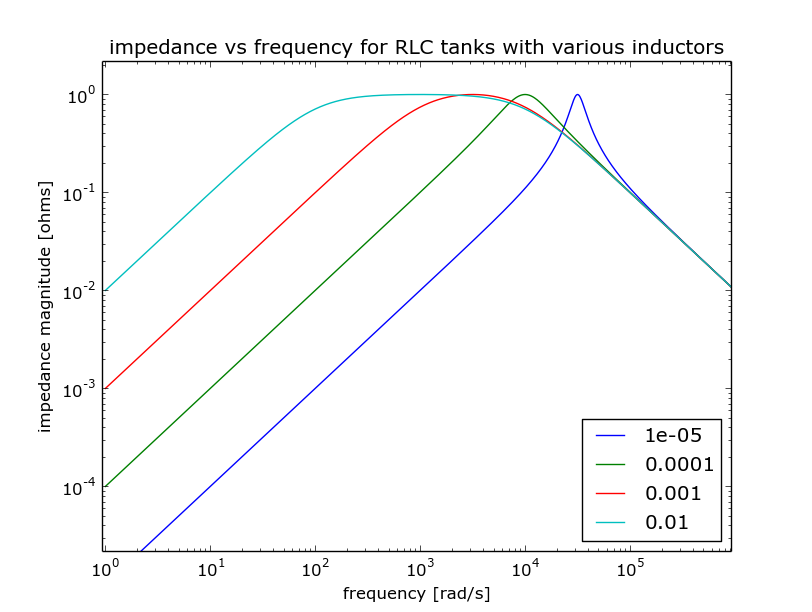
\includegraphics[width=0.35\textwidth]{../inductors.png}
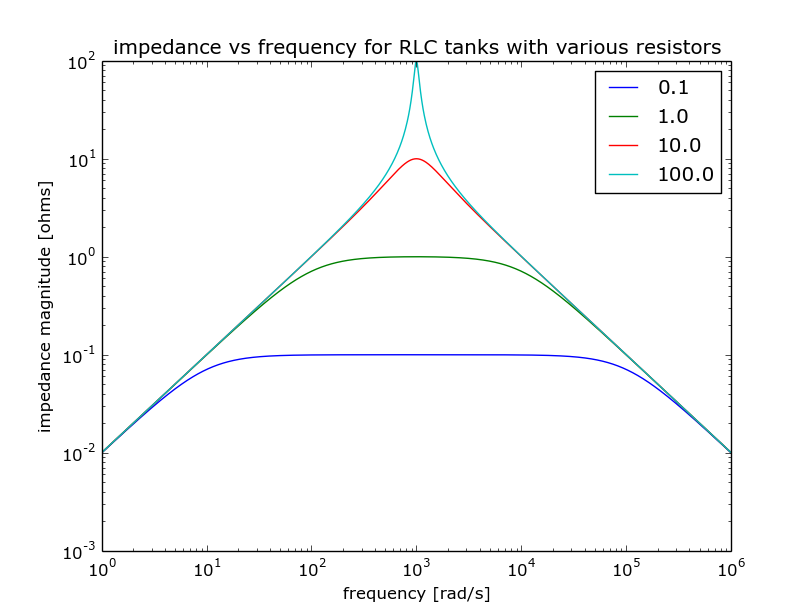
\includegraphics[width=0.35\textwidth]{../resistors.png}
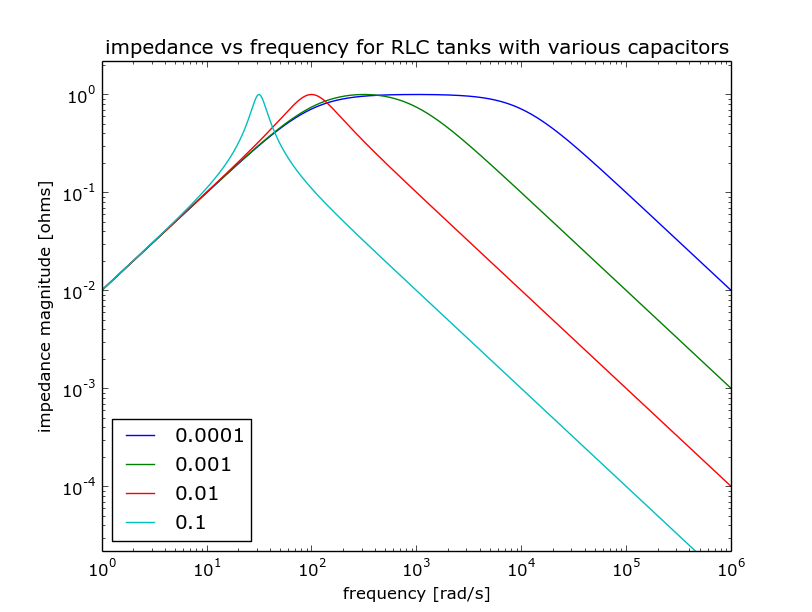
\includegraphics[width=0.35\textwidth]{../capacitors.png}\\
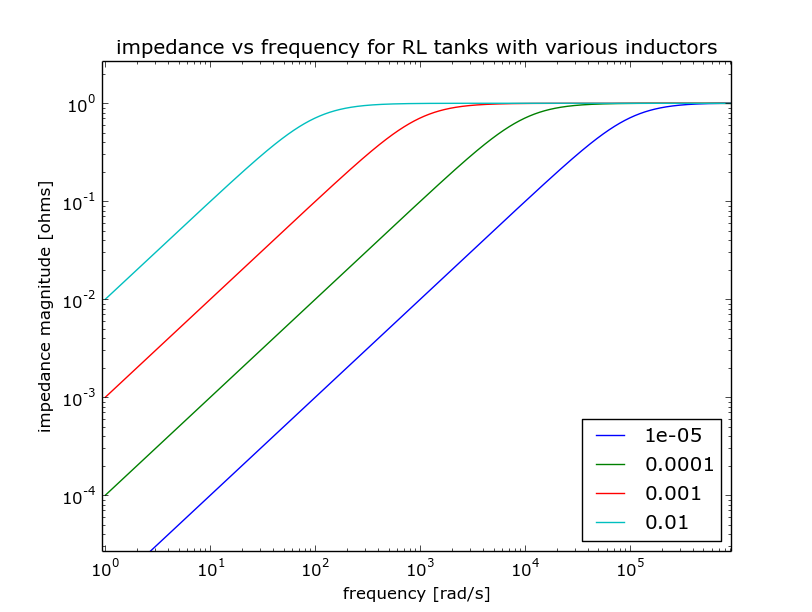
\includegraphics[width=0.35\textwidth]{../rL.png}
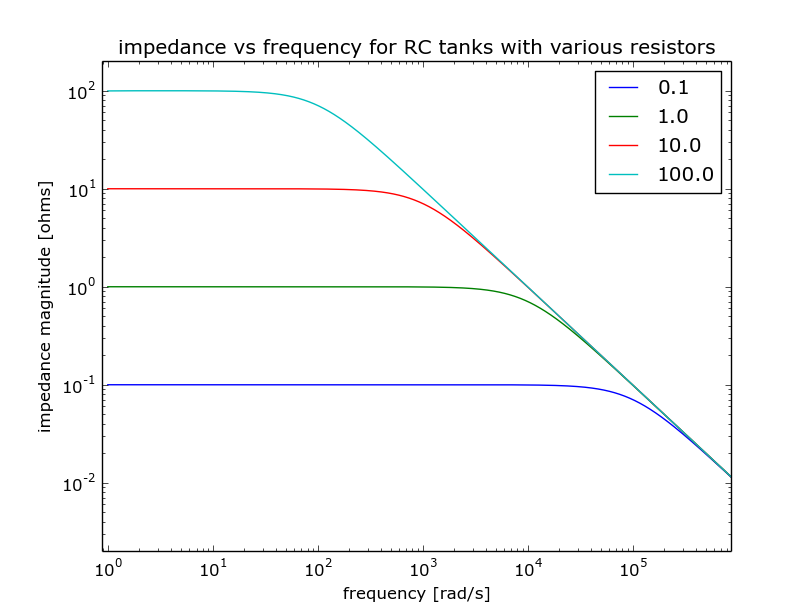
\includegraphics[width=0.35\textwidth]{../Rc.png}
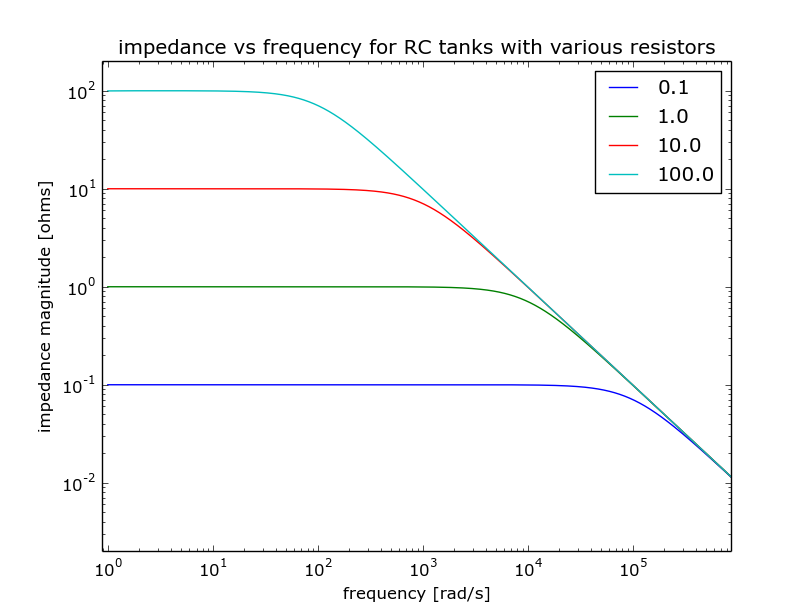
\includegraphics[width=0.35\textwidth]{../rC.png}\\


The plots above illustrate various RLC tank circuits where one component value changes over several orders of magnitude.
In the top-center and bottom-center plots, a decrease in resistance drops the maximum impedance over all frequencies.
In the top-left and bottom-left plots, a decrease in inductance drops the asymptotic impedance at low frequencies
In the top-right and bottom-right plots a decrease in capacitance drops the asymptotic impedance at high frequencies.
As illustrated above, there are three regimes on the impedance vs frequency plot that divide the operation of an RLC tank into three elements:\\
When the slope of \emph{$|Z|$ vs. $f$} is +1, the tank behaves like an inductor with inductance
\begin{equation*}
L=|Z|/(j\omega)
\end{equation*}
When the slope of \emph{$|Z|$ vs. $f$} is -1, the tank behaves like a capacitor with capacitance
\begin{equation*}
C=j\omega |Z|
\end{equation*}
When the slope of \emph{$|Z|$ vs. $f$} is 0, the tank behaves like a resistor with resistance
\begin{equation*}
R=|Z|
\end{equation*}

\subsubsection{Finite Difference Stencil}
To reliably determine the regions of effective resistance, inductance, and capacitance, the slope of the $log{(|Z_{nm}|)}$ vs. $log{(\omega)}$ is computed via the midpoint method.
The midpoint finite difference stencil takes the two points on either side of the point of interest and computes the slope between them.\\
\begin{equation*}
Z'[n]=\frac{1}{2}(Z[n+1]-Z[n-1])
\end{equation*}
\begin{figure}[H]
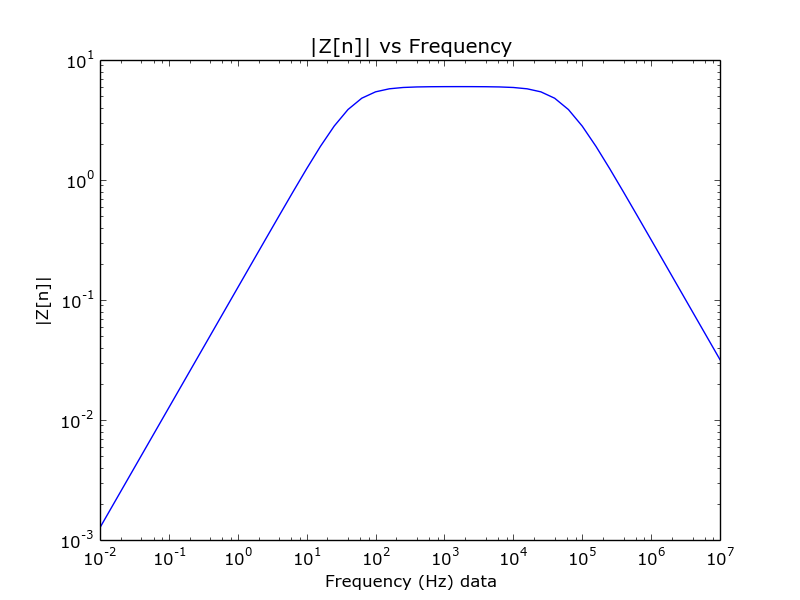
\includegraphics[width=0.5\textwidth]{../fd4.png}
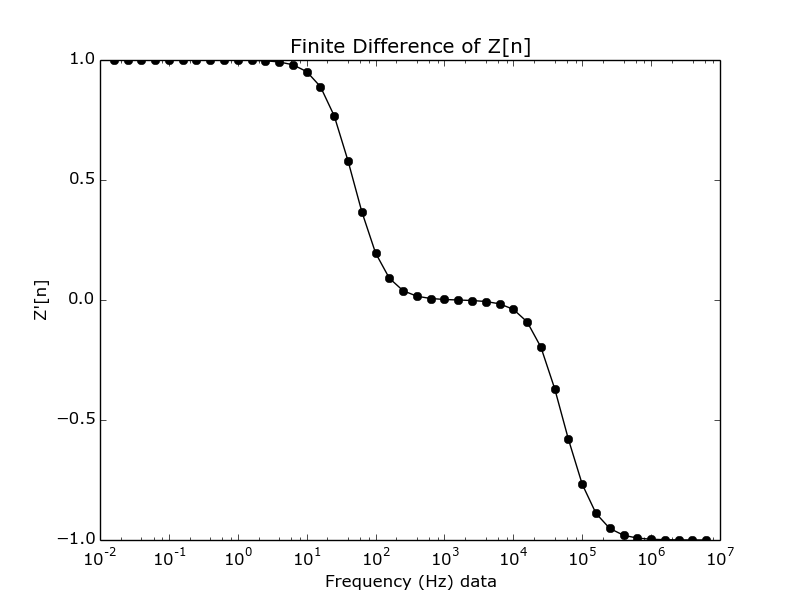
\includegraphics[width=0.5\textwidth]{../fd3.png}
\caption{Finite difference of an RLC tank where R=6$\Omega$, L=20mH, and C=500nF}
\label{fig:fd}
\end{figure}

In figure \ref{fig:fd} the distinct regions of inductance, resistance, and capacitance are clearly visible and easily found by setting thresholds for the finite difference.
The thresholds on the region of inductance are between 1.1 and 0.9, the thresholds on the region of resistance are between 0.1 and -0.1, and the thresholds on the region of capacitance are between -0.9 and -1.1.

\begin{figure}[H]
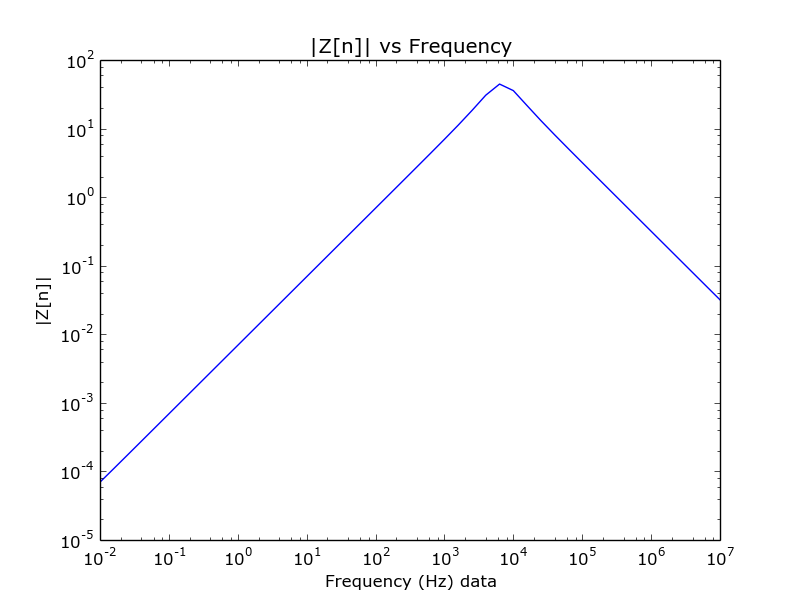
\includegraphics[width=0.5\textwidth]{../fd2.png}
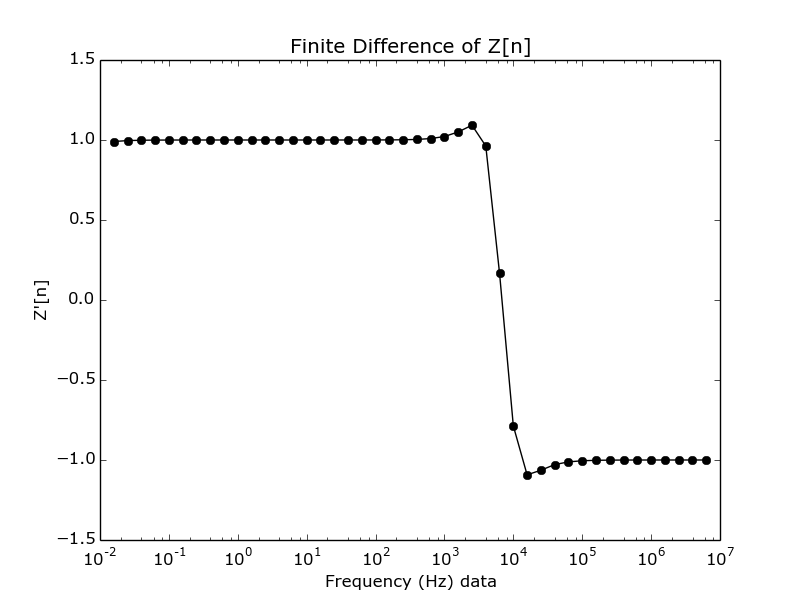
\includegraphics[width=0.5\textwidth]{../fd1.png}
\caption{Finite difference of an RLC tank where R=44$\Omega$, L=1.1mH, and C=500nF}
\label{fig:fd2}
\end{figure}

In figure \ref{fd2}, the resistance is not represented in the finite difference of \texttt{Z[n]}.
The parallel resistance of an underdamped RLC tank is the maximum recorded impedance across all frequencies.
In a simulation, using the maximum recorded impedance is a valid solution because measurement accuracy has a large (64-bit floating point) dynamic range, producing results that are accurate of ideal systems.
In practice, spurious noise and lack of dynamic range over measurement data can cause poor results.
Occasionally these poor results include large spikes of inaccurate impedance readings.
In this case, a practical approach would be to use the finite difference stencil where possible and when an LC network is discovered, sample at the resonant frequency to find R. 
In the case of figure \ref{fig:fd2}, the sampling frequency would be 17KHz.
\begin{equation*}
f_{0} = \frac{1}{\sqrt{2\pi L C}} \approx 17000 Hz
\end{equation*}

\subsubsection{Component Value Calculation}
Once the regions of the impedance plot are thresholded, the sampling frequency domains corresponding to those regions are assigned to an element type [$\omega_r[n]$ for R, $\omega_l[n]$ for L, $\omega_c[n]$ for C].
Then for each sampling frequency the component values are computed and averaged to filter noisy data.
\begin{align*}
R[\omega_r] = Z[\omega_r] \qquad
L[\omega_l] = \frac{Z[\omega_l]}{\omega_l} \qquad
C[\omega_c] = \frac{1}{\omega_c Z[\omega_c]}  
\end{align*}

\begin{align*}
R=\frac{1}{rnum}\sum_{\omega_r}{Z[\omega_r]} \qquad
L=\frac{1}{lnum}\sum_{\omega_l}{\frac{Z[\omega_l]}{\omega_l} \qquad}
C=\frac{1}{cnum}\sum_{\omega_c}{\frac{1}{\omega_c Z[\omega_c]}}
\end{align*}
Where $rnum$, $lnum$, and $cnum$ are the number of sample frequencies in the R, L, and C regions, respectively.

\subsection{Reconstructing the Network}
With a record of all of the elements and their connections in the network, the network can be reconstructed and a schematic of the original circuit can be drawn.

\ifdefined\DEBUG

\section{RLC Elements}

The design of a Network Sensing Algorithm requires an understanding of the networks to be analyzed.
In this thesis, the networks of interest are composed of three circuit elements: resistors, capacitors, and inductors.
The constitutive relations for these electrical circuit elements relate the voltage across an element to the current passing through it as a function of time.
The constitutive relation for resistors, inductors, and capacitors are as follows:

Resistive element behavior is characterized by a linear relationship between current and voltage.
That is, $v=iR$

\begin{figure}[H]
  \begin{center}
    \begin{circuitikz}[american]
		\draw (3,0)
		to[sV,v=$v$,i=$i$] (3,2)
		to[short](5,2)
		to[R=$\displaystyle {R=\frac{v}{i}}$] (5,0)
		to[short](3,0); 
        \end{circuitikz}
   \caption{Constitutive Relations for Resistance}
  \end{center}
\end{figure}

Inductive element behavior is characterized by a linear relationship between the time derivative of current and voltage.
That is, $v=L\frac{di}{dt}$

\begin{figure}[H]
  \begin{center}
    \begin{circuitikz}[american]
		\draw (3,0)
		to[sV,v=$v$,i=$i$] (3,2)
		to[short](5,2)
		to[L=$\displaystyle {L=\frac{v}{\frac{di}{dt}}}$] (5,0)
		to[short](3,0); 
        \end{circuitikz}
   \caption{Constitutive Relations for Inductance}
  \end{center}
\end{figure}

Capacitive element behavior is characterized by a linear relationship between the time derivative of voltage and current.
That is, $i=C\frac{dv}{dt}$

\begin{figure}[H]
  \begin{center}
    \begin{circuitikz}[american]
		\draw (3,0)
		to[sV,v=$v$,i=$i$] (3,2)
		to[short](5,2)
		to[C=$\displaystyle {C=\frac{i}{\frac{dv}{dt}}}$] (5,0)
		to[short](3,0); 
        \end{circuitikz}
   \caption{Constitutive Relations for Capacitance}
  \end{center}
\end{figure}

When combined to form larger networks these constitutive relations hold, but two other laws of conservation are useful for further analysis.

\section{Network Analysis}

\subsubsection{Kirchoff's Current Law}
Kirchoff's current law comes from the idea of conservation of charge.
That is, charge is neither created nor destroyed.
The amount of charge moving along a conductor away from a circuit node is equal to the amount of charge moving along a conductor into that same circuit node.
More succinctly, The sum of the currents going into a node are equal to the sum of currents coming out of that node.

\subsubsection{Kirchoff's Voltage Law}
Kirchoff's voltage law can be derived from conservation of energy.
KVL states that the total amount of energy put into a circuit is equal to the amount of energy lost in that circuit.
Since voltage is a measure of the amount of energy per unit charge, the voltage across a circuit branch is indicative of the amount of energy dissipated as work or provided by an electromotive force.
Following the last two statements, the sum of all of the voltages around a loop in a circuit is zero.

The following sections will use KVL. KCL, and the constitutive relations to reverse-engineer an n-node network.


\end{document}
\fi

\documentclass[12pt,twoside,vi]{mitthesis}
\usepackage{tikz}
\usepackage{circuitikz}
\usepackage{amsmath}
\begin{document}
\chapter{Network Sensing Algorithm}

Given access to the set of nodes in an electrical network, the objective of a network sensing algorithm is to determine the set of branches and the elements that compose them.
In order to illustrate how a network sensing algorithm operates, it is necessary to begin with a simple example and then build in complexity.  

\section{Grounding Clause}

Blah Blah

\section{Two Node Network}
Take the example of a network with two nodes below:

\begin{figure}[h]
  \begin{center}
    \begin{circuitikz}[american]
		\draw (0,3)
		node[label={right:$A$}] {}
		to[R=$R_{AB}$] (0,0)
		node[label={right:$B$}] {};
		\fill (0,3) circle (1mm);
		\fill (0,0) circle (1mm);
		
		\draw (3,0)
		to[short]
		node[sground] {} (3,0);
		\draw (3,0)
		to[V,v=$V_t$,i=$I_t$] (3,3)
		to[short](5,3)
		node[label={right:$A$}] {}
		to[R=${R_{AB}=\frac{V_t}{I_t}}$] (5,0)
		node[label={right:$B$}] {}
		to[short](3,0); 
		
		\draw (9,0)
		to[short]
		node[sground] {} (9,0);
		\draw (9,0)
		to[V,v=$V_t$,i=$I_t$] (9,3)
		to[short](11,3)
		node[label={right:$B$}] {}
		to[R=${R_{BA}=\frac{V_t}{I_t}}$] (11,0)
		node[label={right:$A$}] {}
		to[short](9,0);
		\fill (5,3) circle (1mm);
		\fill (5,0) circle (1mm);
		\fill (11,3) circle (1mm);
		\fill (11,0) circle (1mm);
    \end{circuitikz}
   \caption{Finding $R_{AB}$ in a two node network}
  \end{center}
\end{figure}

In the case of a resistive network with two nodes, there is only one possible branch in the network and thus one possible element to characterize.
From elementary circuit theory, the resistance between two nodes equal to the voltage across the nodes divided by the current through the nodes when power is applied.  
Here, the resistance $R_{AB}$ is found by placing a test voltage $V_t$ across the nodes and measuring the resulting current, $I_t$, then taking the ratio $\frac{V_t}{I_t}$.
This measurement is called the driving point impedance \footnote{To measure a driving point impedance, a test voltage is applied between the node of interest and ground, and the resulting current in the voltage source is measured. 
The driving point impedance is then computed by dividing the test voltage by the resulting current.}.
If there are no circuit elements between the two nodes, the driving point impedance test will find zero current in the test voltage source, resulting in an infinite resistance between two nodes.
An infinite resistance between two nodes in a circuit indicates that there are no elements in that branch of the network.
Thus, the network can subsequently be simplified by removing that branch from the network.


\section{Three Node Network}

A resistive network with two nodes is simple, but provides an introduction to the methodology used in analyzing larger networks.
In the case of a resistive network with three nodes, it is insufficient to utilize driving point impedance measurements alone, because each node has more than one path to any other node.
%Taking the driving point impedance at any node returns a parallel combination of the set of branch resistors, depending on which nodes are grounded.
\begin{figure}[h]
  \begin{center}
    \begin{circuitikz}[american]
    	\ctikzset{label/align = straight}
    	\def\offset{0}
		\draw (\offset,0)
		node[label={above:$A$}] {}
		to[R, l=$R_{AB}$] (3+\offset,0)
		node[label={above:$B$}] {}
		to[R, l=$R_{BC}$] (1.5+\offset,-2.548)
		node[label={right:$C$}] {}
		to[R, l=$R_{AC}$] (0+\offset,0);
		\fill (\offset,0) circle (1mm);
		\fill (1.5+\offset,-2.584) circle (1mm);
		\fill (3+\offset,0) circle (1mm);
		
		\def\offset{5.5}
		\draw (-1+\offset,-2.548)
		to[short]
		node[sground] {} (-1+\offset,-2.548);
		\draw (-1+\offset,-2.548)
		to[V,v=$V_t$,i=$I_t$] (-1+\offset,0)
		to[short](0+\offset,0);
		\draw (\offset,0)
		node[label={above:$A$}] {}
		to[R, l=$R_{AB}$] (3+\offset,0)
		node[label={above:$B$}] {}
		to[R, l=$R_{BC}$] (1.5+\offset,-2.548)
		node[label={right:$C$}] {}
		to[R, l=$R_{AC}$] (0+\offset,0);
		\draw (1.5+\offset,-2.548)
		to[short]
		node[sground] {} (1.5+\offset,-2.548);
		\draw (3+\offset,0)
		to[short] (4+\offset,0)
		to[short] (4+\offset,-2.548)
		node[sground] {};
		\fill (\offset,0) circle (1mm);
		\fill (1.5+\offset,-2.584) circle (1mm);
		\fill (3+\offset,0) circle (1mm);
		
		\def\offset{12}
		\draw (-1+\offset,-2)
		to[short,o-] (-1+\offset,-2.548)
		node[sground] {} (-1+\offset,-2.548);
		\draw (-.75+\offset,-2)
		to[open,v^>=$V_A$] (-.75+\offset,-.1)
		to[open](-1+\offset,0)
		to[short,o-](0+\offset,0);
		\draw (\offset,0)
		node[label={above:$A$}] {}
		to[R, l=$R_{AB}$] (3+\offset,0)
		node[label={above:$B$}] {}
		to[R, l=$R_{BC}$] (1.5+\offset,-2.548)
		node[label={right:$C$}] {}
		to[R, l=$R_{AC}$] (0+\offset,0);
		\draw (1.5+\offset,-2.548)
		to[short]
		node[sground] {} (1.5+\offset,-2.548);
		\draw (4+\offset,-2.548)
		node[sground] {}
		to[V,v_>=$V_t$] (4+\offset,0)
		to[short] (3+\offset,0)
		;
		\fill (\offset,0) circle (1mm);
		\fill (1.5+\offset,-2.584) circle (1mm);
		\fill (3+\offset,0) circle (1mm);
		
    \end{circuitikz}
   \caption{Finding $R_{AB}$ in a three node network}
  \end{center}
\end{figure}

Consider a resistive network with three nodes: A, B, and C. 
In order to determine the resistance in branch AB, the driving point impedance at node A is measured with nodes B and C grounded. 
This provides the resistance of the parallel combination of the branches with an endpoint at node A,\\
$R_{A_{||}} = R_{AB}||R_{AC}$.
\footnote
{$
	\displaystyle R_{1}||R_{2} = 
	\frac{R_{1}R_{2}}{R_{1}+R_{2}}
$}
Next, a test voltage source is applied to node B, node C is grounded, and the voltage at node A, $V_A$, is observed.
$\displaystyle V_{A} = V_t
\frac{R_{AC}} {R_{AB}+R_{AC}} = V_t
\frac{R_{AB}||R_{AC}} {R_{AB}} = V_t
\frac{R_{A_{||}}} {R_{AB}}
$\\
The branch resistance of interest, $R_{AB}$ is calculated using the known quantities $V_t$, $V_{A{||}}$, and $V_A$.
$\displaystyle R_{AB} = 
V_t\frac{R_{A{||}}} {V_A}$ \\
This procedure is repeated for the remaining branches to determine the entire network.


\section{N Node Network}

A resistive network with any number of nodes can be reduced to a resistive network with three nodes by grounding the nodes that are not of interest.
The resulting network does not modify the branch of interest, but connects the remaining branches attached to the nodes of interest in parallel.
This collapses the network into a three node network or three branch equivalent circuit.
\begin{figure}[h]
  \begin{center}
    \begin{circuitikz}
    %\ctikzset{label/align = straight}
		\draw (0,0)
		node[label={above:$A$}] {}
		to[R, l=$R_{AC}$] (1.5,-2.584)
		node[label={below:$C$}] {}
		to[R, l=$R_{EC}$] (3,0) % The resistor
		node[label={above:$E$}] {}
		to[R, l_=$R_{AE}$] (0,0)
		to[R, l^=$R_{AB}$] (-1.5,-2.584)
		node[label={below:$B$}] {}
		to[R, l_=$R_{BC}$] (1.5,-2.584)
		to[R, l_=$R_{CD}$] (4.5,-2.584)
		node[label={below:$D$}] {}
		to[R, l=$R_{ED}$] (3,0);
		\fill (0,0) circle (1mm);
		\fill (3,0) circle (1mm);
		\fill (1.5,-2.584) circle (1mm);
		\fill (4.5,-2.584) circle (1mm);
		\fill (-1.5,-2.584) circle (1mm);
    \end{circuitikz}
   \caption{Five node network}
  \end{center}
\end{figure}
Consider a resistive network with five nodes: A-E.  
To determine the resistance between nodes A and E, the network is reduced to a three-node network by connecting all nodes except nodes A and E to ground.
The three resistances of the branches that remain are $R_{AE}$, $R_{AB}||R_{AC}$, and $R_{EC}||R_{ED}$.
The reduced network is then solved using the three node network method, and this procedure is repeated for all branches in the network.

\section{Element Identification}

Networks composed of elements with complex impedance can be analyzed with the same algorithm.
By replacing the test DC voltage sources with AC voltage sources, the imaginary reactance of capacitors and inductors can be measured in addition to the real resistance of resistors.

\subsection{From Resistance to Impedance}

Chapter 2 described the use of the Laplace Transform to characterize the behavior of circuit elements in the frequency domain.
Here, frequency-domain complex impedance is useful for identifying circuit elements based on the change in branch impedance over inputs of various frequencies.


MAKE NOTE ABOUT USING THE AMPLITUDE OF THE MEASURED SIGNALS

\subsection{Parallel RLC Branches}

To determine if there are multiple element types [in parallel] between two nodes, we can select a few frequencies to scan through and analyze the resulting change in impedance.

\begin{figure}[h]
  \begin{center}
    \begin{circuitikz}
		\draw (0,-.5)
		node[label={below:$2$}] {}
		to[short] (0,0)
		to[R=$R$] (0,2)
		to[short] (1.5,2)
		to[L=$L$] (1.5,0) % The resistor
		to[short] (-1.5,0)
		to[C=$C$] (-1.5,2)
		to[short] (0,2)
		to[short] (0,2.5)
		node[label={above:$1$}] {};
	    \fill (0,-.5) circle (1mm);
		\fill (0,2.5) circle (1mm);
    \end{circuitikz}
   \caption{Example RLC Tank Circuit}
  \end{center}
\end{figure}

The impedance of a parallel RLC 'tank' circuit can be characterized and analyzed over all frequencies.

\begin{align}
Z_C = \frac{1}{j\omega C} \qquad Z_R = R \qquad Z_L = j\omega L \\
Z_{RLC}=Z_C||Z_R||Z_L = \frac{1}{j\omega C+\frac{1}{R}+\frac{1}{j\omega L}}= \frac{j\omega RL}{-\omega^2RLC+j\omega L+R}
\end{align}

$\displaystyle Z_{RLC}$ has a zero at $\frac{1}{RL}$ and two poles at $\frac{-L^{+}_{-}\sqrt{L^2+4R^2LC}}{-2RLC}$\\
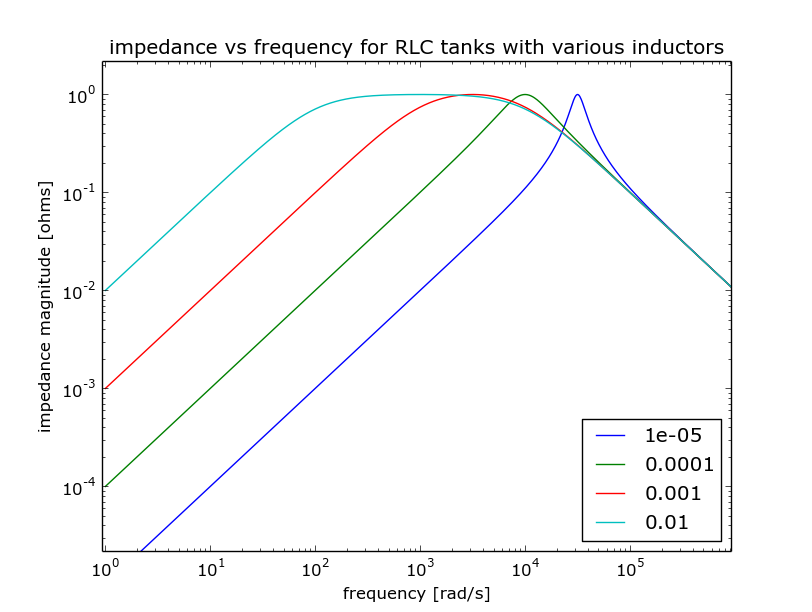
\includegraphics[width=0.35\textwidth]{../inductors.png}
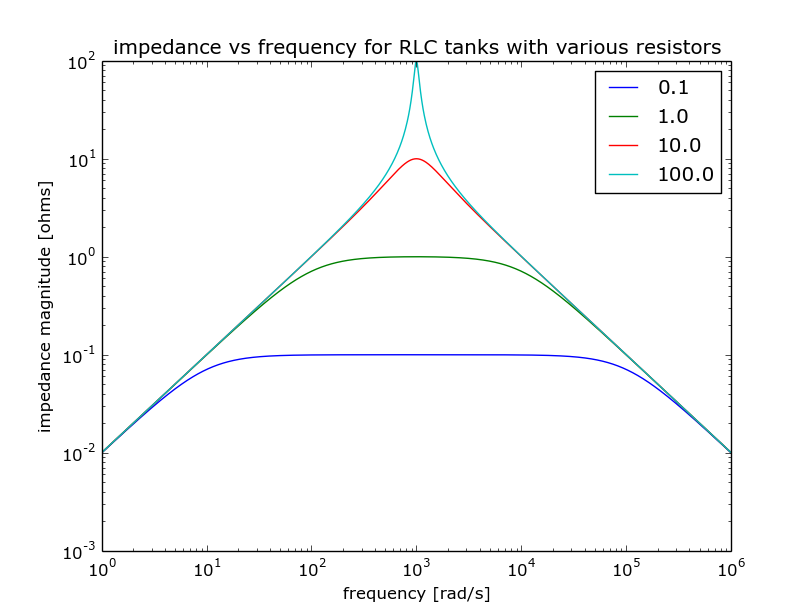
\includegraphics[width=0.35\textwidth]{../resistors.png}
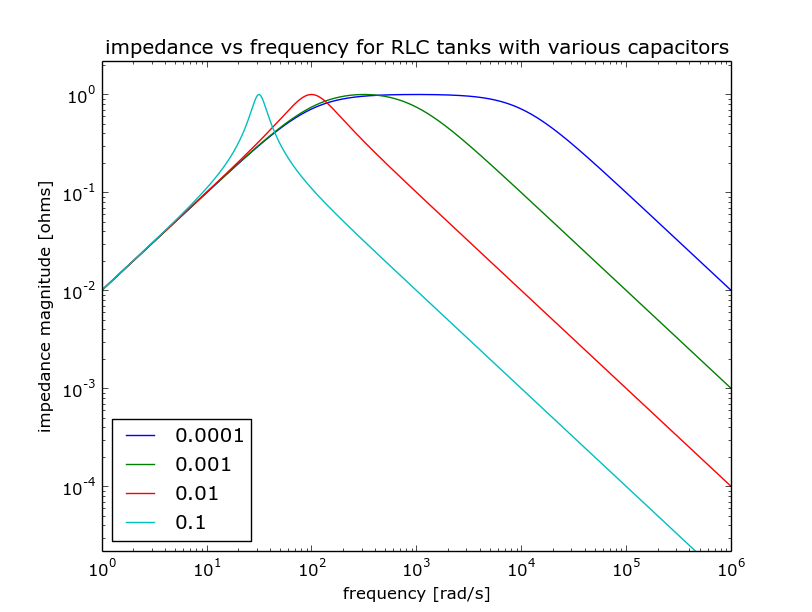
\includegraphics[width=0.35\textwidth]{../capacitors.png}\\
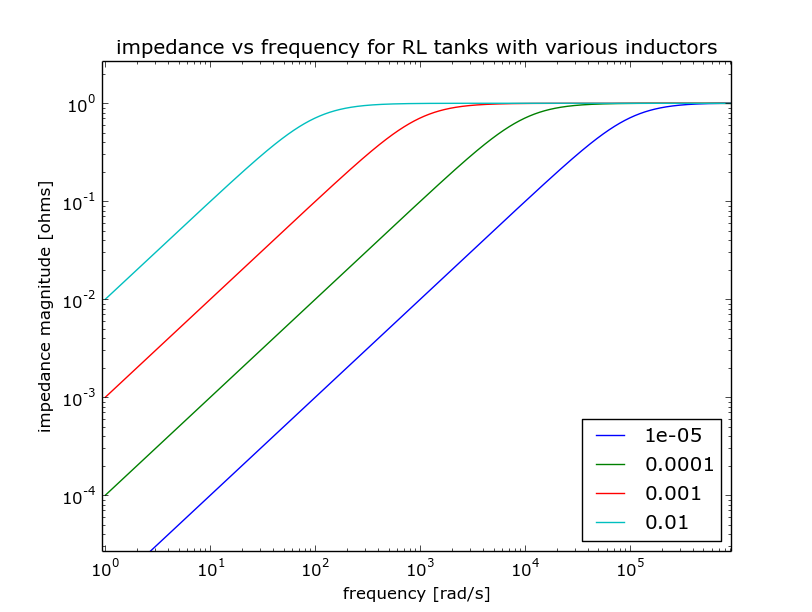
\includegraphics[width=0.35\textwidth]{../rL.png}
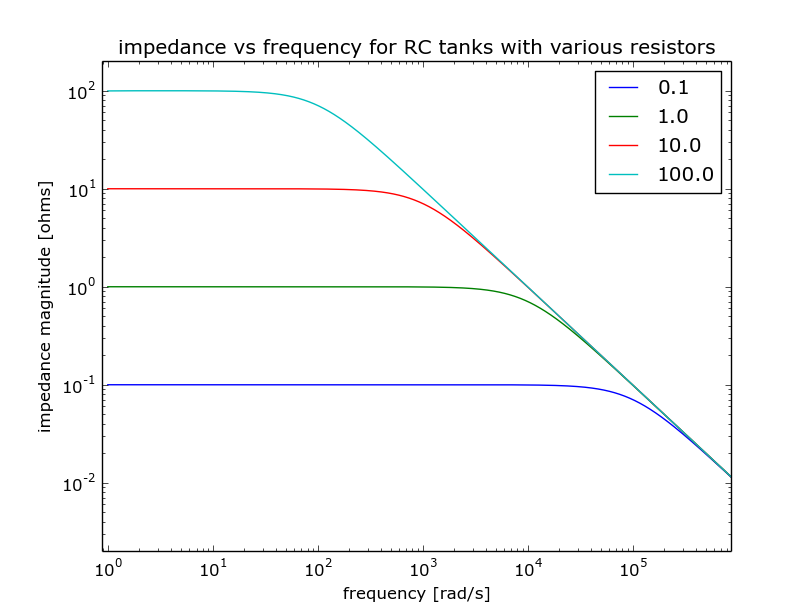
\includegraphics[width=0.35\textwidth]{../Rc.png}
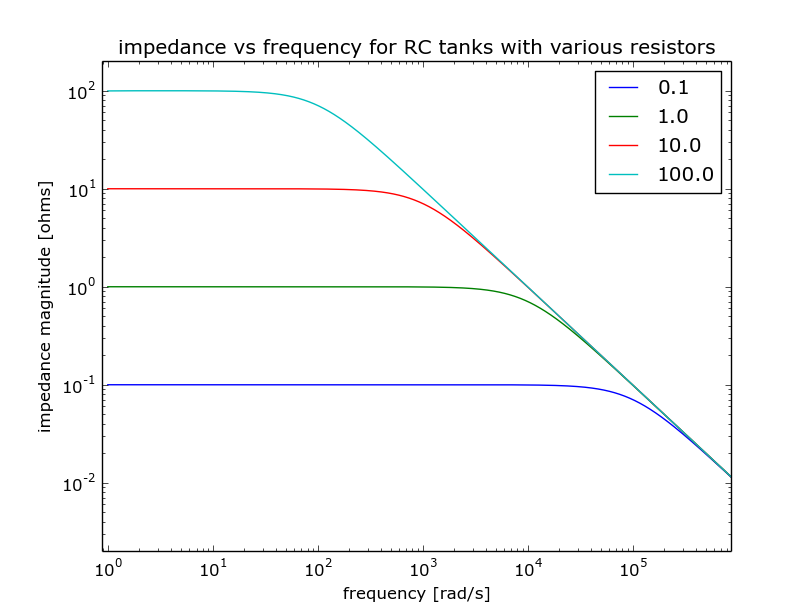
\includegraphics[width=0.35\textwidth]{../rC.png}\\


If we look at the plots above, we can see that varying the resistance changes the maximum impedance over all frequencies, varying the inductance drops the asymptotic impedance at low frequencies, and varying the capacitance drops the asymptotic impedance at high frequencies.
We can imagine there are three regimes on the impedance vs frequency plot that divide the operation of an RLC tank into three elements:\\
When the slope is +1, the tank behaves like an inductor
$L=|Z|/(j\omega)$.
When the slope is -1, the tank behaves like a capacitor
$C=j\omega |Z|$.
When the slope is 0, the tank behaves like a resistor
$R=|Z|$.


\subsection{Finite Difference Stencil}
To reliably determine the regions of effective resistance, inductance, and capacitance, the slope of the $log{|Z_{nm}|}$ vs. $log{(\omega)}$ is computed via the Midpoint Method.
The Midpoint Finite Difference Stencil takes the two points on either side of the point of interest and computes the slope between them.
Z'[n]=$\frac{1}{2}$(Z[n+1]-Z[n-1]).

\subsection{Component Value Calculation}
Once the regions of the impedance plot are identified and assigned to component, the component value is calculated for each sample taken on the impedance plot:\\
$R = Z[\omega]\\
L = \frac{Z[\omega]}{\omega}\\
C = \frac{1}{\omega Z[\omega]} 
$ 

The resulting resistances, inductances, and capacitances are averaged to counter noisy data.


\section{Reconstructing the Network}
With a record of all of the elements and their connections in the network, the network is reconstructed.
\end{document}
%\def\DEBUG{1}
\ifdefined\DEBUG
\documentclass[11pt,twoside]{mitthesis}
\usepackage{tikz}
\usepackage{circuitikz}
\usepackage{amsmath}
\usepackage{fancyvrb}
\usepackage{float}
\newcommand{\ohm}{$\Omega$ }
\begin{document}
\fi


\chapter{Simulation}
In this chapter, a simulation of the circuit sensing breadboard is described.
A simulated circuit sensing breadboard is useful for rapid iteration of hardware topologies and validation of network sensing algorithms.
The simulator is also not limited by the hardware complexity, so simulating circuits with more than eight nodes and elements other than resistors, capacitors, and inductors is possible.
The simulator generates random networks of resistors, inductors, and capacitors, and proceeds to analyze, reconstruct, and draw a schematic of the network using the network sensing algorithm.

\section{NgSpice and Netlists}

The open source software package NgSpice was used to simulate the networks and test circuits applied to the network.
NGspice operates on text files called netlists, where each component in the network is specified on a single line.
An example netlist is shown below.

\begin{figure}[h]
  \begin{center}
    \begin{circuitikz}[american]
    %\ctikzset{label/align = straight}
		\def\offset{0}
		\draw (-1+\offset,-2)
		to[short,o-] (-1+\offset,-2.548)
		node[sground] {} (-1+\offset,-2.548);
		\draw (-.75+\offset,-2)
		to[open,v^>=$V_A$] (-.75+\offset,-.1)
		to[open](-1+\offset,0)
		to[short,o-](0+\offset,0);
		\draw (\offset,0)
		node[label={above:$A$}] {}
		to[R, l=$R_{AB}$] (3+\offset,0)
		node[label={above:$B$}] {}
		to[L, l=$L_{BC}$] (1.5+\offset,-2.548)
		node[label={right:$C$}] {}
		to[C, l=$C_{AC}$] (0+\offset,0);
		\draw (1.5+\offset,-2.548)
		to[short]
		node[sground] {} (1.5+\offset,-2.548);
		\draw (4+\offset,-2.548)
		node[sground] {}
		to[V,v_>=$V_t$] (4+\offset,0)
		to[short] (3+\offset,0)
		;
		\fill (\offset,0) circle (1mm);
		\fill (1.5+\offset,-2.584) circle (1mm);
		\fill (3+\offset,0) circle (1mm);
    \end{circuitikz}
   \caption{Three node network}
  \end{center}
\end{figure}

\begin{Verbatim}[fontsize=\footnotesize]
threeNodeNetlist
Vt	0 B 1
Rab A B 10k
Cac A C 1e-6
Lbc B C 1e-3
Vcg 0 C 0
.control
	op
	print(v(A))
	.endc
.end
\end{Verbatim}

The first letter of each element line designates the element to simulate: \\
\texttt{V start stop value}$\rightarrow$ Voltage Source between \texttt{start} and \texttt{stop} nodes, \texttt{value} Volts [V]\\
\texttt{R start stop value}$\rightarrow$ Resistor between \texttt{start} and \texttt{stop} nodes, \texttt{value} Ohms [$\Omega$]\\
\texttt{L start stop value}$\rightarrow$ Inductor between \texttt{start} and \texttt{stop} nodes, \texttt{value} Henries [H]\\
\texttt{C start stop value}$\rightarrow$ Capacitor between \texttt{start} and \texttt{stop} nodes, \texttt{value} Farads [F]\\

Node 0 is always designated as ground, and all simulations require a ground node.

The control commands are as follows:\\
\texttt{op} $\rightarrow$ Operating Point Simulation
\texttt{print()} $\rightarrow$ Print the relevant data passed as an argument
\texttt{v(N)} $\rightarrow$ The voltage at node N
\texttt{i(E)} $\rightarrow$ The current through element E

\section{Methods}
The NSA simulator was written in python and uses the methods below.

\subsection{Generate Random Netlist}
\texttt{writeRandomNet(netlist,num,elements):}\\
Generates \texttt{num}-node random graph with no self-linking nodes (symmetric matrix with zeros on the diagonal) for each \texttt{[elements]} type (R,L,C).
Subsequently assigns random values between two realistic limits for each element and writes the network to netlist \texttt{netlist}.
1-1k ohms, 10nF-10uF, 100uH-100mH.

When writing the capacitive and inductive elements, care must be taken to prevent a DC operating point simulation from failing.
The infinite resistance across a capacitor and zero resistance across an inductor are responsible for DC operating point simulation failure, and can be fixed by including a small resistor in series with inductors and a large resistor in parallel with capacitors. 

\begin{tabular}{ c c  p{3cm} }
\texttt{L0 1 2 1mH} & $\rightarrow$ & \texttt{L0 1 tl0 1mH Rl0 tl0 2 1e-5} \\
\end{tabular}
\begin{tabular}{ |c  c  p{3cm} }
\texttt{C0 1 2 1e-6F} & $\rightarrow$ & \texttt{C0 1 2 1e-6F Rc0 1 2 1e8} \\
\end{tabular}

\subsection{Inserting Voltage Sources, Grounds and Probes}
\texttt{insertProbe2(target,nodes,groundNodes,probes,source='DC'):}\\
Inserts a 1V voltage source from ground to each node in \texttt{[nodes]}, grounds each node in \texttt{[groundNodes]}, and adds a voltage print statement for each node in \texttt{[probes]}.
By default, the voltage sources are written as DC sources, but if 'AC' is passed into the last argument the sources are written as AC sources and the AC control statement is added.\\
\texttt{AC dec 5 10m 10meg}\\
Which runs a small-signal AC simulation and returns the amplitudes of the resulting voltage and current waveforms, five sample points per decade from 10mHz to 10MHz.

\subsection{Run Simulation}
\texttt{def runSim(target,results,source='DC'):}\\
Makes a system call to NgSpice in batch mode with netlist \texttt{target} and outputs the result to text file \texttt{results}.
The last argument indicates how to parse the resulting data, as NgSpice returns DC data in the following format:
\begin{Verbatim}[fontsize=\footnotesize]
No. of Data Rows : 1
i(v) = -1.18295e-01
v(5) = 2.532846e-07}
\end{Verbatim}
and AC data is returned in this format:
\begin{Verbatim}[fontsize=\footnotesize]
No. of Data Rows : 6
                                   mynetlist
                                   AC Analysis  Sun Aug 30 18:35:07  2015
--------------------------------------------------------------------------------
Index   frequency       i(v)                            
--------------------------------------------------------------------------------
0	1.000000e+00	-1.72598e+00,	3.978810e+02	
1	1.000000e+01	-1.58689e-01,	3.978827e+01	
2	1.000000e+02	-1.43015e-01,	3.974287e+00	
3	1.000000e+03	-1.42859e-01,	3.520201e-01	
4	1.000000e+04	-1.42857e-01,	-4.18884e-01	
5	1.000000e+05	-1.42857e-01,	-4.58275e+00	

                                   mynetlist
                                   AC Analysis  Sun Aug 30 18:35:07  2015
--------------------------------------------------------------------------------
Index   frequency       v(3)                            
--------------------------------------------------------------------------------
0	1.000000e+00	1.000000e+00,	0.000000e+00	
1	1.000000e+01	1.000000e+00,	0.000000e+00	
2	1.000000e+02	1.000000e+00,	0.000000e+00	
3	1.000000e+03	1.000000e+00,	0.000000e+00	
4	1.000000e+04	1.000000e+00,	0.000000e+00	
5	1.000000e+05	1.000000e+00,	0.000000e+00
\end{Verbatim}
DC data is returned as a dictionary with indices for the voltage source current and each node of interest:\\ \texttt{['i':i(V),'1':v(1),'2':v(2),..]}\\
AC data is returned as a dictionary of lists with indices for the voltage source current and each node of interest:\\ \texttt{['i':[i($V_{f_1}$), i($V_{f_2}$),..., i($V_{f_n}$)], '1':[v($1_{f_1}$), v($1_{f_2}$),..., v($1_{f_n}$)], ...]}

\subsection{Print Matrix}
\texttt{def printMatrix(m):}
Prints matrix \texttt{m} in nice command-line output.
It can handle both 2-dimensional and 3-dimensional matrices, for n-by-n matrices with lists of impedances over many frequencies.

\subsection{Write JSON}
\texttt{def writeJSON(name, network,group, elem):}
Writes a JSON file named \texttt{name.json} of the n-by-n symmetric matrix \texttt{network}.
Three separate JSON files are written, one for each element \texttt{[resistor.json, capacitor.json, and inductor.json]}.
The \texttt{group} parameter is used when drawing multiple schematics on one page.
The \texttt{elem} parameter is used to specify what type of element the network represents.

\section{Executing NSA}
\subsection{Calculate $Z_{n{||}}(f)$}
$Z_{n{||}}(f)$ is found by grounding all nodes except for node n and adding a voltage source to that node, then taking the ratio of the amplitudes of the resulting current into the node of interest and the voltage source.
\subsection{Calculate $V_n(f)$}
$V_n(f)$ is found by grounding all nodes except for nodes n and m, adding a voltage source to node m, and measuring the amplitude of the voltage at node n.
\subsection{Calculate $Z_{nm}(f)$}
$Z_{nm}(f)$ is calculated by the ratio of $Z_{n{||}}(f)$ to $V_n(f)$ scaled by $V_t$.
In the case of this simulation, $V_t$ is one.
\subsection{Finite Difference}
$Z_{nm}$ is passed through the finite-differencer, returning a list $Z'_{nm}[f]$.
$Z'_{nm}[f]$ is thresholded to find the frequencies for which $Z'_{nm}[f]\approx-1$, $Z'_{nm}[f]\approx0$, and $Z'_{nm}[f]\approx1$.
\subsection{Element Identification}
A list of inductances is calculated from $Z_{nm}[f]$ on all frequencies for which $Z'_{nm}[f]\approx-1$, $[f_L]$.\\
$\displaystyle L[f_L] = \frac{|Z_{nm}[f_l]|}{(f_l)}$\\
A list of resistances is calculated from $Z_{nm}[f]$ on all frequencies for which $Z'_{nm}[f]\approx0$, $[f_R]$.\\
$\displaystyle R[f_R] = |Z_{nm}[f_R]|$\\
A list of capacitances is characterized from $Z_{nm}[f]$ on all frequencies for which $Z'_{nm}[f]\approx-1$, $[f_C]$.\\
$\displaystyle C[f_C] = \frac{1}{|Z_{nm}[f_C]|(f_C)}$\\

The element lists are averaged to to filter out inaccurate data.

\subsection{Network Reconstruction}

A new matrix is written for each element type, then the matrices are written to JSON and processed by javascript running D3 to display the final schematic.

\ifdefined\DEBUG
\end{document}
\fi

%\documentclass[11pt,twoside]{mitthesis}
%\usepackage{tikz}
%\usepackage{circuitikz}
%\usepackage{amsmath}
%\newcommand{\ohm}{$\Omega$ }
%\begin{document}
\chapter{Hardware}


Block diagram / Schematic


\begin{figure}[h]
  \begin{center}
      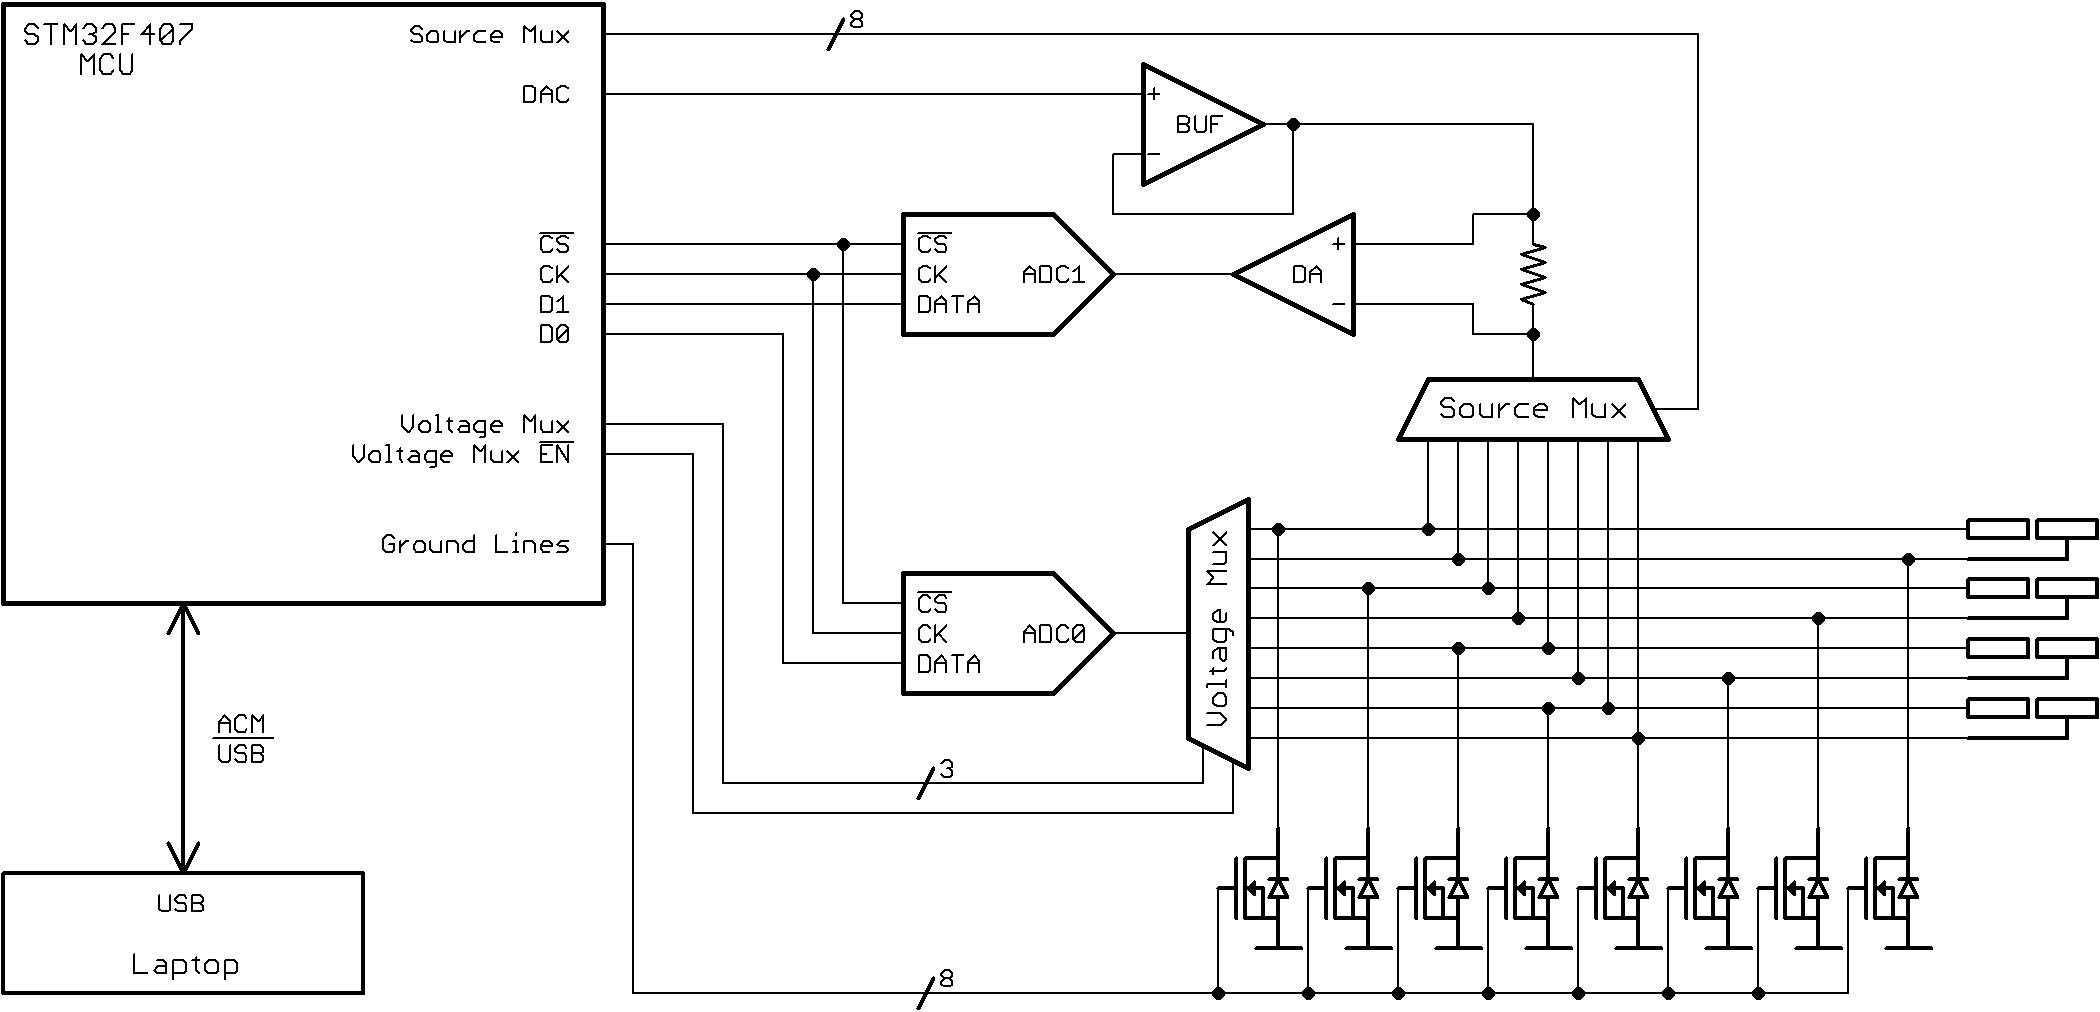
\includegraphics[width=1\textwidth]{../circuit.png}
  \end{center}
\end{figure}
\section{Low Cost}

Keeping the cost of production low makes butterboard accessible to the largest population of people.
Using multiplexed ADCs where possible keeps the cost down by reducing the quantity of high price-tag components, like ADCs.

\section{Node Voltage Reading}
An ADCS7476 12-bit A/D converter is used to measure the voltages at each node.
The ADCS7476 can sample up to 1MSPS with $\pm$1 LSB of total unadjusted error from $-40^o C$ to $85^o C$ and $<\pm 0.2$ LSB of error at $25^o C$.
No bits are wasted in the ADCS7476 A/D converter.
Additionally, the input circuitry to the ADC is a 100$\Omega$ resistor in series with a 26pF capacitor.  
This places a pole at 61MHz, causing a .03\% error at 100KHz and .3\% error at 1MHz.
The additional performance is well worth the additional cost of \$1.56375 in quantities of 1Ku.

\begin{figure}[h!]
  \begin{center}
      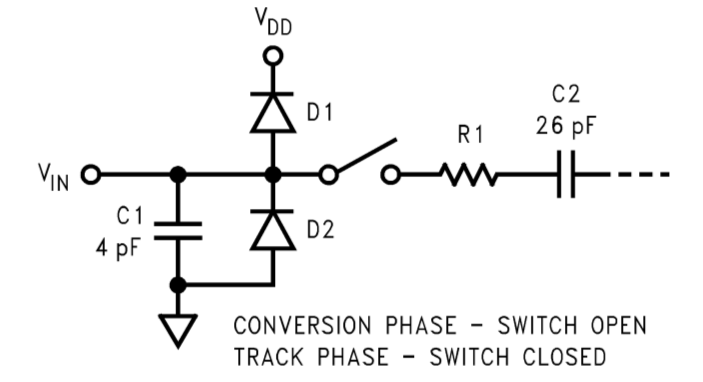
\includegraphics[width=.5\textwidth]{../adc-input-equiv.png}
      \caption{ADCS7476 Equivalent Input Circuit}
  \end{center}
\end{figure}


The ADC is connected to the common pin of a CD4051 1:8 analog multiplexer.
The multiplexer is connected to eight breadboard rails, which allows the ADC to measure the voltage on any of the eight rails, one rail at a time.

The CD4051 has about $200\Omega$ of series resistance and 30pF of output capacitance when its supply voltage is 12V, which places an additional pole at 26MHz, again well above the Nyquist frequency.

So far, the voltage-reading signal chain has two poles - one at 61MHz and one at 26MHz.

\subsection{Onboard A/D converters}
Although the STM32F407 has three onboard 12-bit A/D converters, their specifications are lacking.
Each is able to sample at 2MSPS, and it's possible to interleave them to attain a sampling rate of 6MSPS or higher if you're willing to throw away bits.
The total unadjusted error (offset error, gain error, differential linearity error, and integral linearity error) is between $\pm$2 LSB and $\pm$5 LSB.
With a minimum of $\pm$2 LSB's of error, the lowest significant two bits in the 12-bit A/D are virtually useless.
Another specification to consider is the input circuitry to the ADC.
The input circuitry to the ADC while it's in tracking mode looks like a 6K$\Omega$ resistor charging a 4pF capacitor.
This puts a pole at 6.6MHz, causing .3\% error in measurement at 100KHz, 3\% error in measurement at 1MHz, and 7\% at 3MHz.
When sampling at the maximum sample rate of 6MSPS, the ADC's input network begins to introduce significant error.
Granted, it's likely that there will be an alternative bandwidth bottleneck, this is still a metric of concern.
[DM00037051.pdf, pages 133-134]

\section{Signal Generator}

The STM32F407 has an onboard D/A converter that is good enough to use as a signal generator.
The onboard DAC is configured to output a cosine wavetable with a DC offset, as described in the next chapter.

\section{Test Voltage Current Sensing}

The DAC output is buffered by half of an MCP6L92 10MHz op-amp.
The onboard DAC can be configured with an optional onboard buffer, but the buffer limits the DAC output range from 0.2V to Vdd-0.2V.
Without the onboard buffer, the DAC output is 15k$\Omega$.
When configured as a voltage buffer, the MCP6L92 has an input impedance larger than 1G$\Omega$, resulting in no signal attenuation.

\begin{figure}[h!]
  \begin{center}
      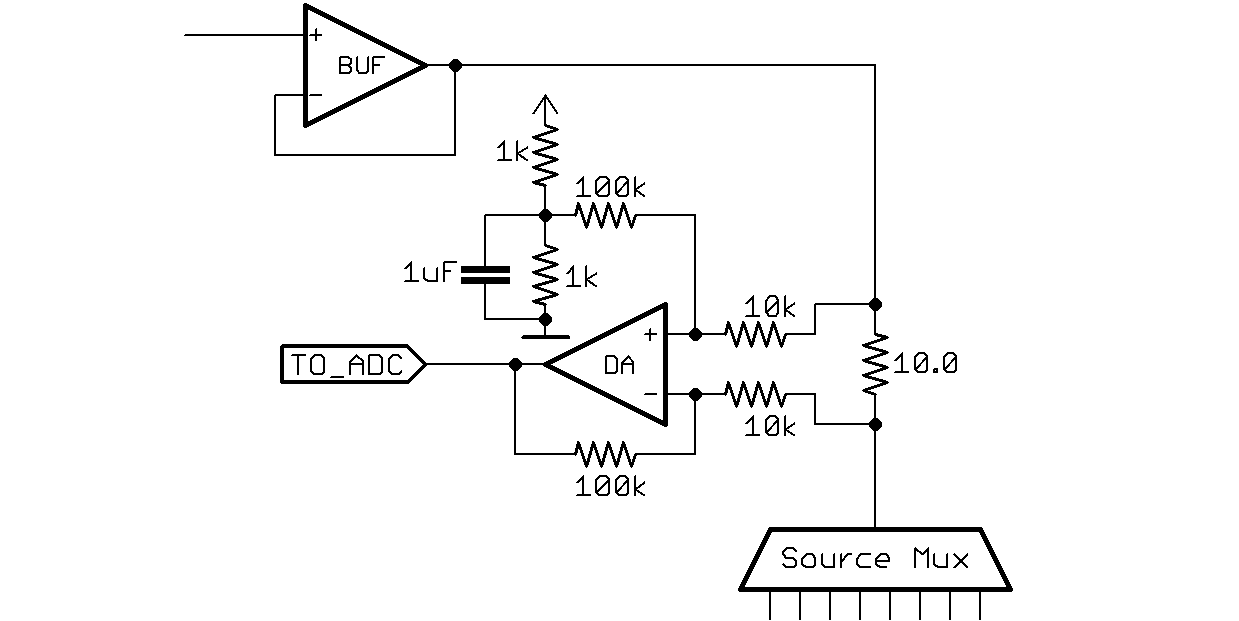
\includegraphics[width=.7\textwidth]{../DA.png}
      \caption{Difference Amplifier Schematic}
  \end{center}
\end{figure}

The buffer sources current through a 10.0\ohm, 1\% sense resistor, which can be switched onto any of the breadboard rails through an array of eight high-side switches.
The voltage across the sense resistor is measured by the other half of the MCP6L92 op-amp configured as a simple difference amplifier.
Using two 10k\ohm resistors and two 100k\ohm resistors, the difference amplifier is configured with a gain of 10.  

\begin{figure}[h!]
  \begin{center}
      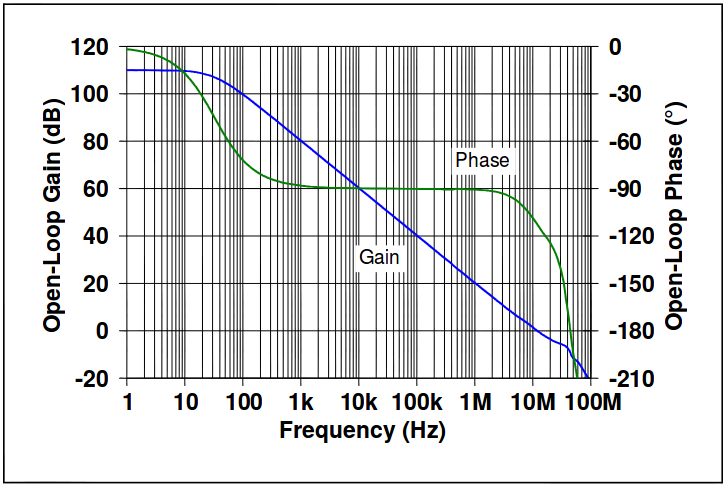
\includegraphics[width=.6\textwidth]{../opamp-bode.png}
      \caption{MCP6L92 Open Loop Bode Plot}
  \end{center}
\end{figure}

According to the MCP6L92 datasheet, the difference amplifier should have a -3dB bandwidth of 1MHz and plenty of phase margin driving the 100\ohm - 26pF input impedance to the current sense ADC.


\section{High-side Switches}

The high-side switches were selected for high-voltage operation, so that any rail of the breadboard could swing between 0 and 30V and there wouldn't be a problem.
The selected switches were Vishay DG468 normally open analog switches.
They have 9\ohm resistance and 76pF of capacitance in the on-state, 1nA of leakage current and 30pF of capacitance in the off-state.
The high and low side switches are the main limits of bandwidth due to their high amounts of input capacitance in both on and off states.


\section{Low-side Switches}

The low-side switches have a low logic-level threshold voltage, low drain-source on-resistance, can handle up to 30V, and are low-cost.
The IRLML2803 N-FETs have an $R_{DS_{ON}}$ of about 1\ohm with a $V_{GS}$ of 3.3V.
With 10V $V_{GS}$, $R_{DS_{ON}}$ drops to 250m\ohm.
The downside of these FETs is the high $C_{DS}$ that comes from a wide transistor.
$C_{DC}$ is on the order of 60pF for each transistor.
When combined with the additional capacitances mentioned above, each breadboard rail has a total of 140pF to ground.  
This has a significant impact on the maximum usable frequency for even moderate impedances on the breadboard.
For example, consider a 10k\ohm-10k\ohm resistor divider.
At 100kHz, the 140 pF capacitance on each rail has 11k\ohm of impedance.
\begin{figure}[h]
  \begin{center}
    \begin{circuitikz}[american]
    %\ctikzset{label/align = straight}
	
		\draw (0,0)
		node[sground] {}
		to[V,v^>=$V_t$] (0,3)
		to[short] (2,3)
		to[R,l_=$10k\Omega$] (2,1.5)
		to[R,l_=$10k\Omega$] (2,0)
		to[short] (0,0);
		\draw(2,1.5)
		to[short] (4,1.5)
		to[C,l_=$140pF$] (4,0)
		to[short] (2,0);
		\fill (2,1.5) circle (1mm);
		
		\draw (8,0)
		node[sground] {}
		to[V,v^>=$V_tsin(100KHz)$] (8,3)
		to[short] (10,3)
		to[R,l_=$10k\Omega$] (10,1.5)
		to[R,l_=$10k\Omega$] (10,0)
		to[short] (8,0);
		\draw(10,1.5)
		to[short] (11,1.5)
		to[R,l=$11k\Omega$] (11,0)
		to[short] (10,0);
		\fill (10,1.5) circle (1mm);
		
    \end{circuitikz}
   \caption{Resistor Divider Parasitic Capacitance}
  \end{center}
\end{figure}

\section{PCB Mounted Breadboard}

\section{Hardware Prototypes}
%\end{document}

\chapter{Firmware}
Block Diagram

\section{Fast and Scalable [rename]}
16 1MSPS ADCs all at once, multiplexed out.

\section{ADC}
\subsection{ADC Timers}
\subsection{ADC DMA}
\subsection{Data Reconstruction}

\section{DAC}
\subsection{DAC Timer}
\subsection{DAC DMA}
\subsection{DAC Wavetables}

\section{USB}
\subsection{USBACM}
\subsection{Command List}

\chapter{Software Control}

\section{Control Routine}

"Just a teaspoon of sugar makes the medicine go down" - Mary Poppins



\subsection{Data Reconstruction}
10-bits from 8-bit serial data

\section{Finding Amplitude}
\subsection{Tracking Method?}
This one didn't work so well.
\subsection{FFT}
Yeah, this one works real well.

\section{Node Iteration Loop}
\subsection{Sampling}
\subsection{Finite Differencing}
\subsection{Resistor Characterizing}

\section{JSON Update}


%\def\DEBUG{1}
\ifdefined\DEBUG
\documentclass[11pt,twoside]{mitthesis}
\usepackage{tikz}
\usepackage{circuitikz}
\usepackage{amsmath}
\usepackage{fancyvrb}
\usepackage{float}
\newcommand{\ohm}{$\Omega$ }
\begin{document}
\fi

\chapter{Results}
In this chapter, results for the simulation and hardware implementations of the RLC network identifying system are presented and analyzed.
The shortcomings of the systems are addressed and potential improvements are discussed as future work.

\section{Simulation Performance}
The performance of the RLC network identification system simulator is analyzed by its output precision and cases in which it fails.
The output precision of the simulator is quite good and can be controlled almost arbitrarily.
The precision depends almost entirely on the thresholds defined during the finite-differencing step, as looser thresholds allow bad data to get averaged into the good data.
The cases in which the simulator fails are always cases where a relatively high resistance is in parallel with an LC network.
In these cases, the simulator reports that there is no resistor in parallel with the LC network.
The failure mode lies within finite difference stencil thresholding, where the simulator never finds a region where the slope of the impedance vs frequency plot is zero, and in turn the simulator decides there is no resistor.
Designing a better element identifying algorithm would make excellent future work.

The schematic renderer used to display the returned matrices as a legible schematic could use some work as well.
It is effective at creating schematics for circuits composed of resistors with only a few nodes, but the value labeling system and lack of organization quickly gets out of hands when the number of nodes is greater than five.
There has been a fair bit of research into auto-generating schematics from netlists, particularly from the days of discrete digital logic, such as \emph{ASG [Automatic Schematic Generator]} from Lageweg at Delft University \cite{delft} and the \emph{ASG} from Jehng, Chen, and Parng at National Taiwan University \cite{taiwan}.


%This could be remedied by either a patch to the algorithm or another algorithm entirely.
%Instead of using a slope of zero on the \texttt{|Z| vs. f} plot to indicate parallel resistance, the maximum recorded impedance can be taken as the parallel resistance whenever the simulator finds an LC circuit.
%In the case of an LC circuit where there is no resistance, 

\section{Hardware Performance}

The hardware RLC network identification system was tested to determine its dynamic range of operation, precision, and ability to detect RLC networks.

\subsection{Element Testing}
\subsubsection{Resistance}
A selection of resistors ranging from 33\ohm to 330k\ohm were analyzed with the RLC network identification system.  
For each resistor, the identified resistance was recorded and plotted. 

\begin{figure}[H]
	\label{fig:rplot}
  \begin{center}
      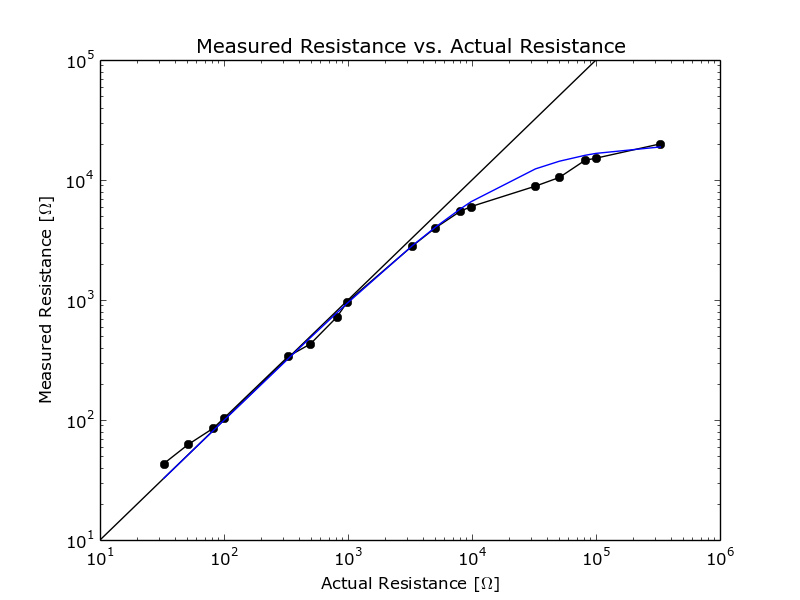
\includegraphics[width=.7\textwidth]{../rin-ro.png}
      \caption{Plot of measured resistance for known resistors}
  \end{center}
\end{figure}

From the Figure \ref{fig:rplot}, the range of resistances for which the system maintains valid precision operation is between $\sim100$ and 2000\ohm.
For resistances larger than 2k\ohm, the system returns resistances that are far smaller than the input resistance.
The asymptotic portion of the curve in Figure \ref{fig:rplot} indicates a parallel resistance somewhere around 20k\ohm.
The blue line indicates the equivalent resistance of each tested resistance with a parallel 20k\ohm resistor.
This parallel resistance is not real.
Using an ohmmeter, it was verified that there is not enough leakage current between breadboard nodes or between breadboard nodes and ground to account for 20k\ohm of resistance.
Rather, this measurement error is caused by the minimum non-zero signal amplitude measured on the output of the current amplifier A/D converter.
A 10-bit ADC that samples a $5V$ window converts every $.004V$ into one bit.
The minimum amplitude signal produced by a 10-bit ADC sampling over a $5V$ scale has an amplitude of $4mV$.
The test voltages applied to each node have amplitudes around $0.75V$.
The current amplifier has a gain of 100, so the effective current amplitude measured is $40\mu A$. 
\quad \qquad \qquad \qquad \qquad \qquad $0.75V / 40\mu A=18750\Omega$\\
So, the maximum possible impedance measurement from any node to ground, $R_{n_{||}}$, is 19k\ohm.
A frequency sweep of the impedance of an open node, such as the one in Figure \ref{fig:zopen}, demonstrates this.
\begin{figure}[H]
	\label{fig:zopen}
  \begin{center}
      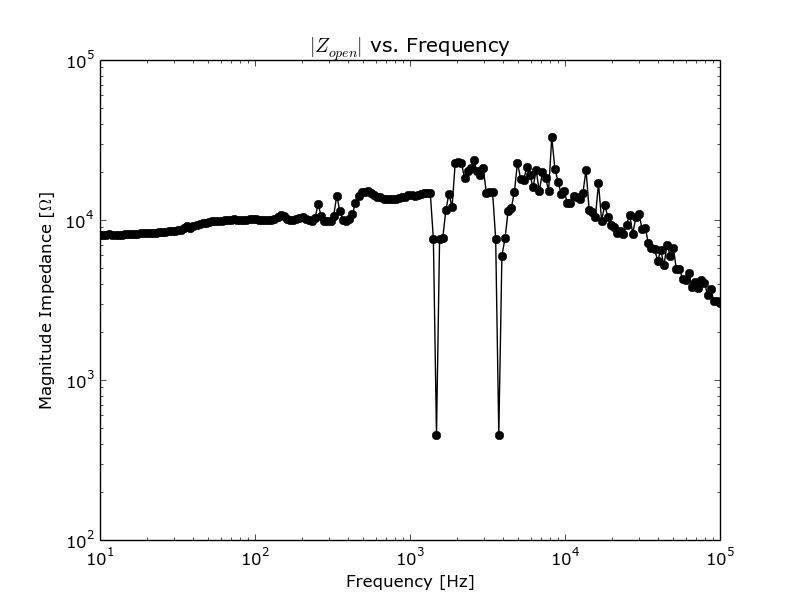
\includegraphics[width=.7\textwidth]{../zopen-gnd.png}
      \caption{Driving point impedance of an open node from 1Hz to 100KHz}
  \end{center}
\end{figure}
By adding a variable gain stage to the current amplifier, or a variable-sized sense resistor, the maximum impedance measurement could be modified.

The maximum impedance measurement between two nodes, rather than just one node to ground, is an order of magnitude higher.
This is due to the procedure used in the network sensing algorithm, where $V_t R_{n_{||}}$ is divided by $V_m$.
If $V_n$ is smaller than 1, the resulting resistance $R_{nm}$ is larger than $R_{n_{||}}$

\begin{figure}[h]
	\label{fig:z2open}
  \begin{center}
      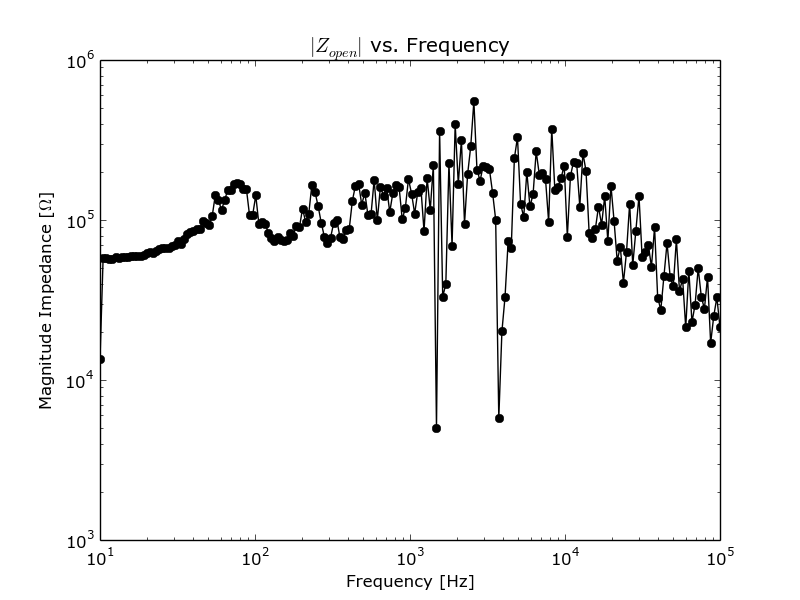
\includegraphics[width=.7\textwidth]{../zopen.png}
      \caption{Impedance between two open nodes from 1Hz to 100KHz}
  \end{center}
\end{figure}

On the other side of Figure \ref{fig:rplot}, for resistances smaller than 100\ohm the system returns resistances that are far larger than the input resistance.
This can be attributed to the DAC buffer current limit, which is $\pm25mA$.
For a test voltage signal of $\sim1.5V$, a 60\ohm resistance produces a $25mA$ current.
This agrees with the recorded data quite well.
To measure resistances smaller than 100\ohm the output buffer could be replaced with one that has a higher output current limit.
Alternatively, a variable-sized sense resistor would also mitigate the problem.

\subsubsection{Capacitance}

In addition to the resistors, a selection of capacitors ranging from $220pF$ to $22\mu F$ were analyzed with the RLC network identification system.  
For each capacitor, the identified capacitance was recorded and plotted in Figure \ref{fig:cplot}.

\begin{figure}[h]
	\label{fig:cplot}
  \begin{center}
      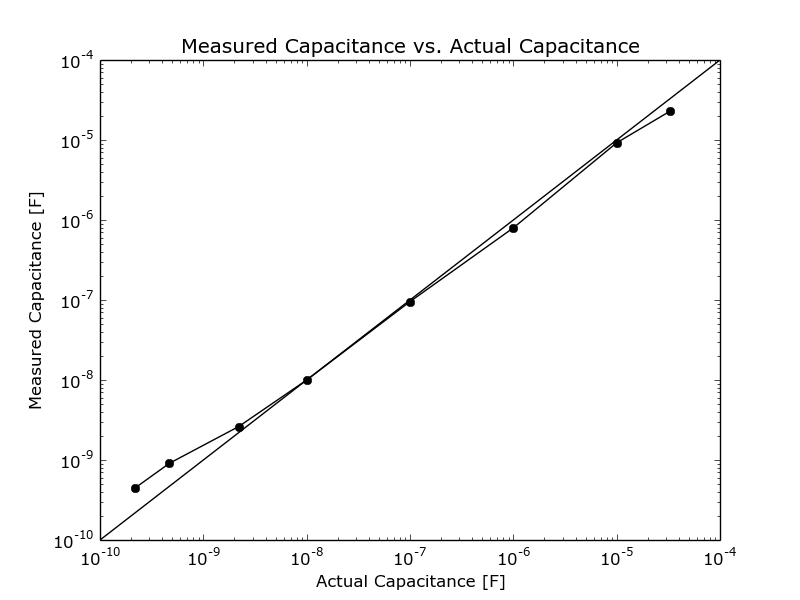
\includegraphics[width=.7\textwidth]{../cin-co.png}
      \caption{Plot of measured capacitance for known capacitors}
  \end{center}
\end{figure}

The RLC network identification system can precisely measure capacitances over three orders of magnitude, from $2.2nF$ to $10\mu F$.
On the low end of Figure \ref{fig:cplot}, the parallel parasitic capacitance is visible, which adds about $150pF$ to the system, although this does not entirely account for the measured capacitance.
On the high end, the impedance of the capacitors at the test frequencies drops below 50\ohm, again causing the buffer op-amp to reach its output current limits and saturate.
The working range of $1nF$ to $10\mu F$ is acceptable for general purposes.

\subsubsection{Inductance}



A selection of inductors ere analyzed with the RLC network identification system to no avail.
The identification system was not able to find the inductors due to the noisy nature of the impedance measurements that inductors were found to return.


The 'noisy' impedance, shown in Figure \ref{fig:lplot}, defeats the finite-differencing technique, and causes it to return a large (amplitude of 20) random-looking signal.
This is much larger than the +1 output that is expected for an inductor, and causes the element identification step to fail.

In addition to recording noisy measurements while attempting to identify an inductor alone, noisy measurements were found when attempting to identify RL, LC, and RLC parallel circuits.
One would expect to find noisy inductive data in the section of the plot where the inductor dominates and and clean capacitive or resistive data in the sections of the plot where the capacitor or resistor dominates, but this is not the case.
This issue has not been closed, yet is integral to the acceptable operation of an RLC network identification system.
Identifying and solving this problem would make excellent future work.

\begin{figure}[h]
	\label{fig:lplot}
  \begin{center}
      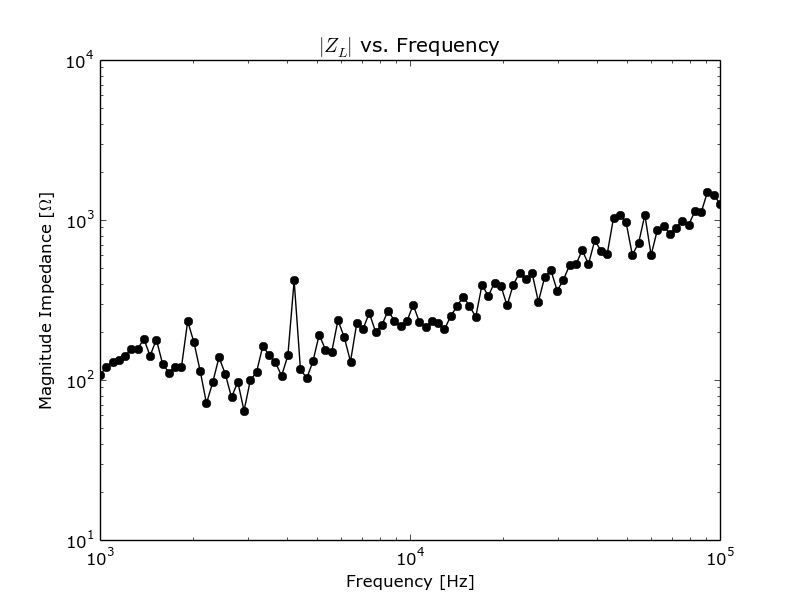
\includegraphics[width=.7\textwidth]{../zl.png}
      \caption{Impedance vs frequency for a $3.3mH$ inductor, demonstrating inductive behavior albeit noisily}
  \end{center}
\end{figure}

\begin{figure}[H]
	\label{fig:lcplot}
  \begin{center}
      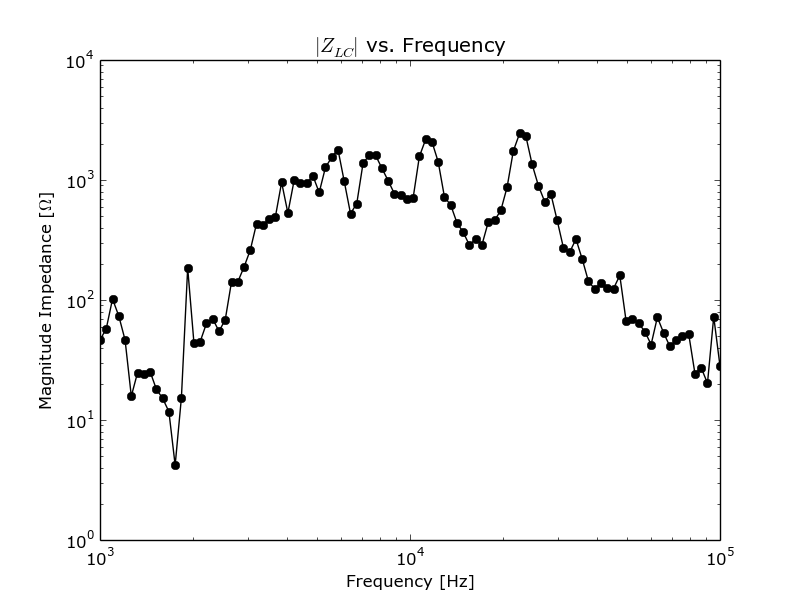
\includegraphics[width=.7\textwidth]{../zlc.png}
      \caption{Impedance vs frequency for a $3.3mH$ inductor in parallel with a $0.15\mu F$ capacitor, demonstrating LC behavior albeit noisily}
  \end{center}
\end{figure}
\newpage
\subsection{Network Testing}

\subsubsection{Resistive Networks}
To verify the network identification system performed properly, complete networks of three, four, five, and six nodes were constructed from resistors within the range of 100\ohm to 1000\ohm.

\begin{figure}[H]
	\label{fig:nodes}
		\begin{center}
      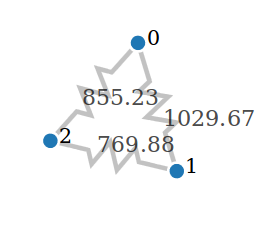
\includegraphics[width=.4\textwidth]{../3node.png}
      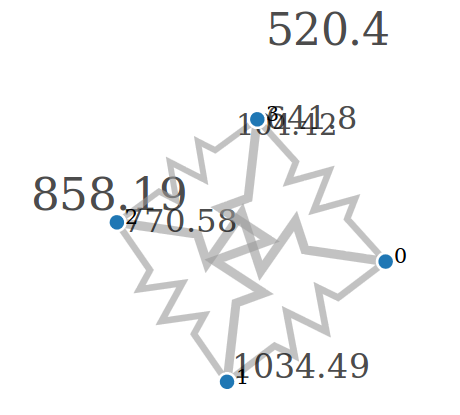
\includegraphics[width=.4\textwidth]{../4node.png}
      \end{center}
      \begin{center}
      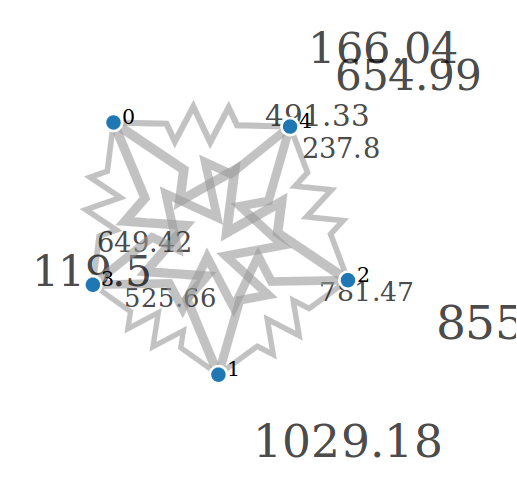
\includegraphics[width=.4\textwidth]{../5node.png}
      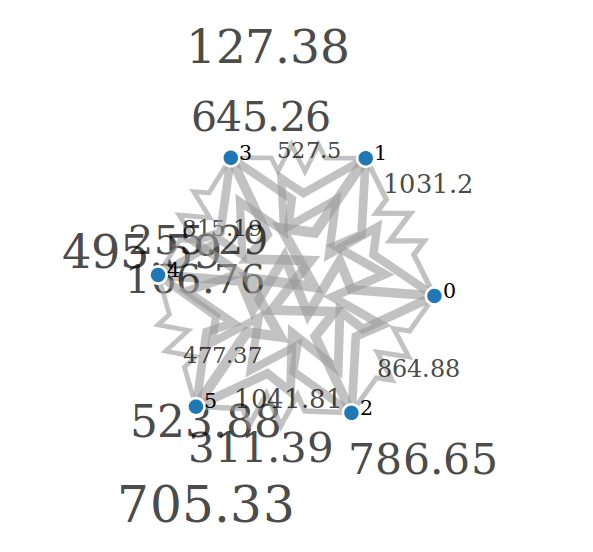
\includegraphics[width=.4\textwidth]{../6node.png}
      \end{center}
      \caption{Schematics of 3, 4, 5, and 6-node resistor networks rendered in the browser}
\end{figure}

The RLC network identification system successfully detected all of the resistive connections in the complete 3, 4, 5, and 6 node networks.
However, many of the values were detected with more than 5\% error once the network became large.
This error is produced by the nonlinear weighting that occurs when combining resistors in parallel.
As the network grows, each $R_{n_{||}}$ measurement contains more resistive elements in parallel with the branch of interest.
If all of these resistive elements are on the same order of magnitude in value ($R$, the additional attenuation due to the addition of another parallel resistor goes as $\frac{k}{k+1}$, if k is the current number of resistors.
This causes error in the measurement of $R_{nm}$ to be amplified by $R(k+1)$

\begin{align*}
R_{nm}'&= \frac{V_t R_{n_{||}}}{V_n} \qquad from ~ Section ~ 2.1.3\\
&= \frac{\frac{r_{nm}}{R+r_{nm}}}{\frac{1}{R+R_{nm}}}
\end{align*}
with error $\Delta_r$, $\Delta_v$:
\begin{align*}
R_{nm}' &= \frac{V_t R_{n_{||}}}{V_n} = \frac{\frac{R_{nm}}{R+k R_{nm}}+\Delta_r}{\frac{1}{R+kR_{nm}}+\Delta_v}\\
&= \frac{R_{nm}+\Delta_r (R + k R_{nm})}{1+\Delta_v(R+kR_{nm})}
\end{align*}
If $R_{nm}\approx R$, error contributed by $R_{n_{||}}$ measurements is $\Delta_r R (k+1)$ and the error contribued by $V_n$ measurements is $\frac{1}{1+\Delta_v R (k+1)}$, both of which are scaled by the number of parallel resistances.
To improve performance in the cases where many branches connect to one node, improve measurement precision and dynamic range.
In the previous tests, the average resistance was $\sim500$\ohm.
Five 500\ohm resistors' equivalent parallel resistance is 100\ohm, close to the lower bound on the identification system's dynamic range.
This analysis explains the asymmetry found in many of the measured resistance matrices, since each node had different parallel equivalent resistances, $R_{n_{||}}$.

The following data correlates to the test networks in Figure \ref{fig:nodes}.
Column index $i$ and row index $j$ are node numbers, the value at at index $i,j$ is the resistance $R_{ij}$.

\begin{Verbatim}[fontsize=\footnotesize]
N=3
R measured                          R actual
None     1.03e+03 8.55e+02                   1.00e+03 8.20e+02
1.03e+03 None     7.70e+02          1.00e+03          7.50e+02	
8.56e+02 7.71e+02 None              8.20e+02 7.50e+02     
\end{Verbatim}


\begin{Verbatim}[fontsize=\footnotesize]
N=4
R measured                                R actual
None     1.03e+03 8.58e+02 6.42e+02                1.00e+03 8.50e+02 6.20+e02
1.03e+03 None     7.71e+02 5.20e+02       1.00e+03          7.50e+02 5.10e+02
8.63e+02 7.84e+02 None     1.04e+02       8.50e+02 7.50e+02          1.00+e02
6.46e+02 5.27e+02 1.04e+02 None           6.20e+02 5.10e+02 1.00e+02     
\end{Verbatim}

\newpage 

\begin{Verbatim}[fontsize=\footnotesize]
N=5
R measured                                     R actual
None     1.03e+03 8.56e+02 6.49e+02 4.91e+02            1.00e+03 8.50e+02 6.20e+02 5.10e+02
1.04e+03 None     7.81e+02 5.26e+02 1.66e+02   1.00e+03 None     7.50e+02 5.10e+02 1.60e+02
9.99e+02 8.87e+02 None     1.19e+02 2.38e+02   8.50e+02 7.50e+02          1.00e+02 2.00e+02
6.66e+02 5.31e+02 1.05e+02 None     6.55e+02   6.20e+02 5.10e+02 1.00e+02          6.20e+02
5.02e+02 1.67e+02 2.10e+02 6.54e+02 None       5.10e+02 1.60e+02 2.00e+02 6.20e+02 
\end{Verbatim}

\begin{Verbatim}[fontsize=\footnotesize]
N=6
R
None     1.03e+03 8.65e+02 6.45e+02 4.96e+02 5.24e+02  
1.04e+03 None     7.87e+02 5.28e+02 1.67e+02 7.05e+02  
1.06e+03 9.65e+02 None     1.27e+02 2.55e+02 1.04e+03  
8.10e+02 6.60e+02 1.31e+02 None     8.15e+02 3.11e+02  
5.57e+02 1.91e+02 2.39e+02 7.67e+02 None     4.77e+02  
5.19e+02 6.97e+02 8.51e+02 2.49e+02 4.12e+02 None     
\end{Verbatim}

\subsubsection{RC Networks}
Similar results are found when measuring RC networks.

\section{Improvements}
Various improvements would be welcome future work.
From design focused on individual subsystems to topological changes, there is much to improve on this iteration of a circuit sensing breadboard.
\subsection{Variable Gain Amplifiers}
Adding a Variable Gain Amplifier to the ADC, DAC, and current sense amplifier signal chains would enable a large increase in dynamic range of the entire system.
Not only would it improve the resolution (and thus precision) of measuring elements on the far-ends of the dynamic range, but it would enable higher resolution captures of small signals, improving the overall utility of the device.

\subsection{Variable Sense Resistor}

Similar to the aforementioned improvement, this would improve the dynamic range and resolution of the current measurements.  

\subsection{Better Switches}
The switches in this system are the main contributors the high parasitic capacitance between every node and ground.
The parasitic capacitance causes undesired attenuation of signals at high-frequencies, making This version of the circuit sensing breadboard unsuitable for even moderate-frequency circuit design.
Finding switches with lower parasitic capacitances would likely require permitting higher $r_{DS_{on}}$, which is possible but requires further testing.
Alternative technologies for switches, such as relays, seem promising as they have very low parasitic capacitance and low on resistance, at the cost of bulk.

\subsection{Better Schematic Display}

The schematic display was built on top of D3, a javascript library for graphical applications in the browser.
D3 was chosen because of its large community and available relevant example code.
In particular, \emph{Force Graph}.
Force graph is interesting because it could be configured to take an arbitrary graph and simulate a kind of spring fabric between the nodes.
Nodes tied together with edges are attracted to one another, but nodes not connected repel.
This action 'unfolds' random networks until they appear flat, with as few crossing branches as possible.
Replace the branches with resistors, capacitors, and inductors and voilia!
Unfortunately, using a relatively unmodified version of force graph in this application makes schematic display design lacking in many facets.
Namely, lack of well-placed labels, trouble with handling parallel components, lack of orientation, and lack of visual control.
Redesigning the current schematic display or designing a new one would greatly improve the usability of the system.

\subsection{Additional Devices}

At the moment, the RLC network identification system can only identify resistor and capacitor networks with a maximum of eight nodes.
Designing a system that can successfully identify inductors would be a huge improvement.
Additionally, determining how to identify systems composed of more complex components like diodes, transistors, transformers, and even integrated circuits is an interesting and likely rewarding problem to solve.

\subsection{Computer-Aided Debugger}

Although the intent of this hardware system is to display a live schematic of a circuit under construction, the hardware is capable of serving other purposes.
Take, for example, a system that is given the schematic of the circuit at hand.
The circuit is performing unexpectedly, so the circuit symptom is reported to the system.
The system, knowing what the circuit should be, computes how the circuit should behave.
Now, since the system knows how the circuit should behave, it asks the user to probe various parts of the circuit, comparing its simulation of the circuit to the actual signals on the circuit.
Mismatches in simulated and physical signals are traced to their sources, and the bug is found.
If the system were also give electrical access to every node in the circuit, it may also be able to debug the circuit on its own.
This would make excellent future work.

\section{Conclusion}

A system that draws a live schematic of a resistive circuit built on an eight-rail breadboard was presented and analyzed.
The system was decomposed into its algorithmic, hardware, firmware, and software components, each of which were described in detail.
A new method for mounting breadboards to printed circuit boards was prototyped and presented.
The performance of the overall system was measured and analyzed, and much was learned along the way.
Although RLC network identification systems may not be feasible, realistic, or desirable, future work on this topic could lead to some interesting and novel systems.

\ifdefined\DEBUG
\end{document}
\fi
\appendix
%\chapter{Tables}

\begin{table}
\caption{Armadillos}
\label{arm:table}
\begin{center}
\begin{tabular}{||l|l||}\hline
Armadillos & are \\\hline
our	   & friends \\\hline
\end{tabular}
\end{center}
\end{table}

\clearpage
\newpage

%\chapter{Figures}

\vspace*{-3in}

\begin{figure}
\vspace{2.4in}
\caption{Armadillo slaying lawyer.}
\label{arm:fig1}
\end{figure}
\clearpage
\newpage

\begin{figure}
\vspace{2.4in}
\caption{Armadillo eradicating national debt.}
\label{arm:fig2}
\end{figure}
\clearpage
\newpage

%%% This defines the bibliography file (main.bib) and the bibliography style.
%% If you want to create a bibliography file by hand, change the contents of
%% this file to a `thebibliography' environment.  For more information 
%% see section 4.3 of the LaTeX manual.
\begin{singlespace}
\bibliography{main}
\bibliographystyle{plain}
\end{singlespace}

\end{document}

